% !TEX TS-program = latex
\documentclass[a4paper,12pt]{report}
\newcommand{\ra}[1]{\renewcommand{\arraystretch}{#1}}
\usepackage{amsmath}
\usepackage[mathscr]{eucal}
\usepackage{amssymb}
\usepackage{indentfirst}
\usepackage{latexsym}
\usepackage{hyperref}
\usepackage{setspace}
\usepackage{enumerate}
\usepackage{pdfpages}
\usepackage{url}
\usepackage{verbatim}
\usepackage{booktabs}
\usepackage{color}
\usepackage{epsfig}
\usepackage{longtable}
\usepackage{tabularx}
\usepackage{dcolumn}

\usepackage{float}
\usepackage{xspace}

\newcommand{\todo}[1]
{
    {\color{red}$\bigstar$~\textsf{#1}\\}
}

\newcommand{\todosub}[1]
{
    {\color{blue}$\triangleright$~\textsf{#1}\\}
}

\newcommand{\tododone}[1]
{
    {\color{red}$\checkmark$~\textsf{#1}\\}
}

\newcommand{\EditOne}[1]
{
    {\color{blue}{#1}}
}


\newcommand{\K}{{\tt Kepler}}


\bibliographystyle{plain}
\textwidth=14.945cm
\oddsidemargin=0.5cm
\evensidemargin=0.5cm

\begin{document}
\doublespacing

\begin{titlepage}
\vspace*{2cm}
\noindent
\begin{flushleft}
	\setlength{\baselineskip}{2\baselineskip}
	{{\Huge \bf Automatic Classification of Kepler Planetary Transit Candidates Using Artifical Neural Network}}
\end{flushleft}


\vspace{1cm}
\vspace{\fill}
\vspace{1.3cm}
\begin{tabbing}
mmmmmmmmmmmmmmmmm\= \kill
\>Prabath Peiris\\
\>Capstone Project\\
\>Machine Learning Nanodegree\\
\>Udacity\\
\> \\
\end{tabbing}
\end{titlepage}

\thispagestyle{empty}
\newlength{\origpar}
\setlength{\origpar}{\parindent}
\setlength{\parindent}{0pt}
%\input{Abstract/abstract}
\setlength{\parindent}{\origpar}
\thispagestyle{empty}
\tableofcontents
\clearpage

\renewcommand {\baselinestretch} {1.0}
\pagebreak
%\pagenumbering{arabic}


\chapter{Introduction}

\tododone{Introduction}

%%%%%%%%%%%%%%%%%%%%%%%%%%%%%%%%%%%%%%%%%%%%%%%%%%%%%%%%%%%%%%%%%%%%%%%

Kepler is a space observatory launched by NASA in 2009 to discover Eath-sized exoplanets orbiting other stars  \cite{2010ApJ...713L..87J}. Kepler mission developed several decades to answer the centuries-old question: How frequent are other Earth-like planets in Milkyway galaxy? In particular, what is the frequency of Earth-size planets in the Habitable-Zone of solar-like stars? There are three different types of exoplanets are common in our universe: gas giants, hot-super-Earths in short period orbits, and ice giants. The challenge is to find the terrestrial planets that are in the habitable zone of their host stars where liquid water might exist on the surface of the planet.

The scientific objective of the Kepler mission is to explore the structure and diversity of planetary systems. This mission surveys a large sample of stars to determine the percentage of terrestrial and large planets that are in or near the habitable zone of a wide variety of stars and determine the distribution of size and shapes of the orbits of these planets. Kepler mission also estimates how many planets are in multiple-star systems. After collecting a large number of data points, using many techniques scientists determine the properties of those stars that harbor planarity systems including the planets itself. 

After preprocessing raw data, the goal is to classify each detection into one of the three different categories: Planetary Candidate (PC), Astrophysical False Positive (AFP) and None transiting phenomena (NTP ). Historically this process is done by researchers looking at each observation. This is a very slow and time consuming process. During this project, I am attempting to automate this classification process using machine learning algorithms.

\section{Search for Earth-Like Planets}
\tododone{What Problem we are solving - Project Origin, Background problem domain}
\tododone{- define the problem : explain in detail about the exoplanets}
One of the most fundamental and intriguing philosophical questions has remained for at least 2300 years is whether life exists outside of our Solar System. With the science and technology has grown exponentially within the last couple of hundred years, it is now, we have the theoretical knowledge, practical and feasibility to seek answers to this question from a scientific perspective. NASA's Navigator Program is the long term project that over-seeing the missions related to  detecting and characterization of Earth-like planets. These missions consist of multidisciplinary suite of research efforts, centering on finding exoplanets that could harbor biological activity similar to terrestrial life.

In the process of searching for Earth-like planets, we will encounter a spectrum of planets. The planetary population conceivably outnumbers stellar population since a star could host many planets such as our solar system. Unlike stars\footnote{Vogt-Russell theorem states that the properties of a star are fully determined by the mass and chemical composision.}, planets can have many different characteristics, careful examination of the planets in our solar system show us that full understanding of planets, in general, requires a working knowledge of diverse fields including star formarion, orbital mechanics, geology, grophysics, climatology, agronomy, chemistry, biology and various engineering disciplines. 

we need to address a couple of questions in the search for habitable worlds:

\begin{itemize}
	\item How do planetary systems form and evolve?
	\item Are there other planetary systems like our own?
	\item Is there life elsewhere in the Universe?
\end{itemize}

Search for habitable planets begins with an understanding of the formation of planetary systems in protoplanetary disks to learn how planetary systems form, around which types of stars planets form, how often planets form, and how the disk properties effect the distribution of final planets sizes and orbits\cite{2002ApJ...580..494Y}.The primary mission for observing the formation of planetary systems will be the James Webb Space Telescope (JWST) \cite{Gardner2006}. JWST will allow us to study the earliest moments of star and planet formation. 

In the quest of finding an extraterrestrial life form, the current observations suggest that Earth-sized rocky planets may be common; however, their abundance is quite uncertain. Kepler is a one the space-based mission\cite{2010ApJ...713L..87J} that is under NASA's navigator program which observes planetary systems in our solar neighborhood. Kepler also finds correlations between the presence of Eath-like planets and both stellar characteristics and the presence and orbits of giant planets. It is important to understand that no single instrument or technique is capable of finding all planetary system components around stars of all ages. Many space and ground bases missions will use complementary instrumentations and techniques to explore majority of planetary discoveries. There are four fundamental techniques will be used to determine the architecture of planetary systems: (i) \emph{Radial Velocity Measurements} (ii) \emph{Transit Observations}, (iii) \emph{Astrometry} (iv) \emph{Direct Detection}.

To answer the question ``Is there life elsewhere in the universe?'', we need to look for habitable planets. For us to determine whether a planet is habitable, we must build observations capable of directly detecting the light from the planet, with the planet illuminated by the light from its parent star. Direct detection of these planets is an enormous technical challenge. Another way to infer habitability of a planet is to check if the planet is located in the \emph{Habitable Zoned} of the host star. Habitable Zone is the range in the distance from a star where liquid water could exist on the surface of a planet orbiting a star that possibly supports life. Liquid water is essential to all life on Earth, and so the definition of a habitable zone is based on the hypothesis that extraterrestrial life would share this requirement \cite{2014ApJ...787L..29K}. This is a very traditional definition, as a planet surface temperature may depend on other factors such as greenhouse gas abundance, its reflectivity, atmospheric and oceanic circulation, radioactive decay, and tidal heating within the planet. These energy sources can be easily allowed the planet to have subsurface liquid water reservoirs.  Jupiter's moon Europa has liquid water ocean tens of kilometers below its surface that may well be habitable for some organisms. More than 20 planets, including the nearest extrasolar planet, Proxima Centauri b \cite{2016Natur.536..437A}, have been found that are both roughly Earth-sized and orbiting within a Habitable Zoned of their stars. 


\begin{figure}[!h]
\begin{center}
        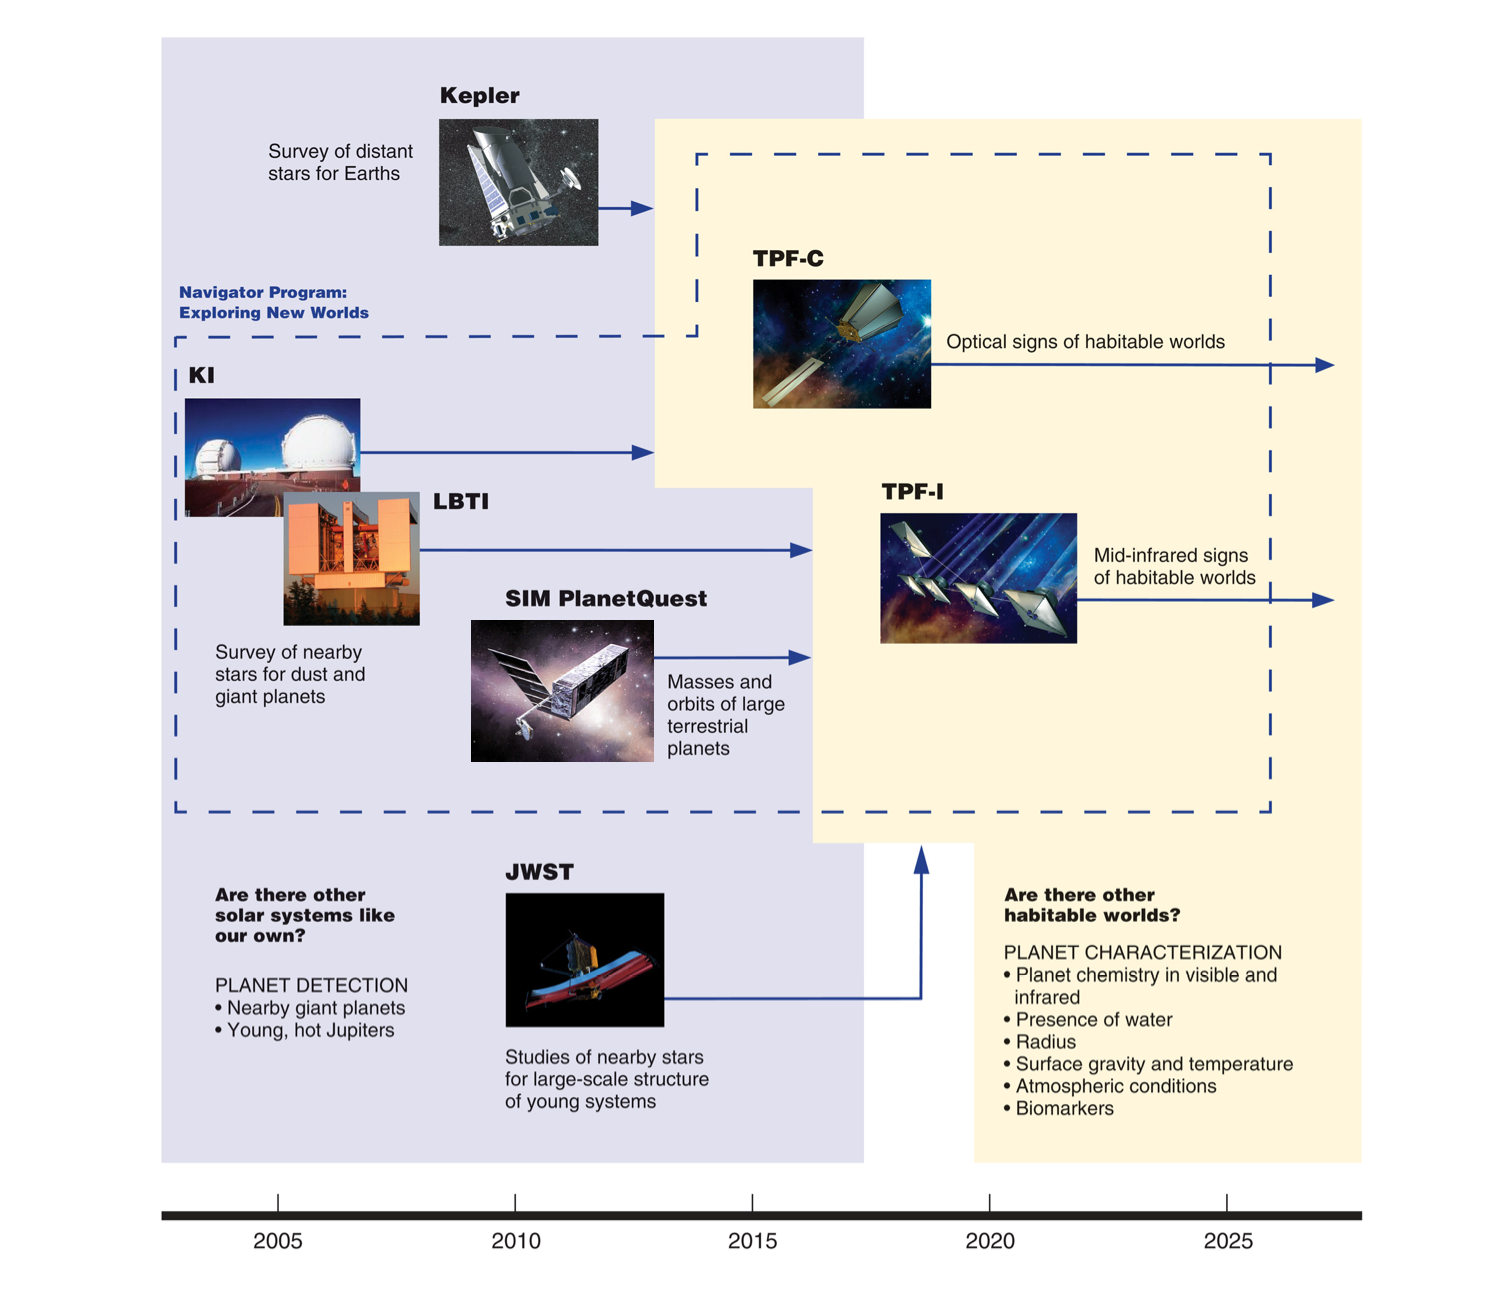
\includegraphics[width=0.8\textheight]{img/navigatorprogram.png}
        \caption{Navigator Program. National timeline including the flow of science between missions, including the \emph{Kepler} Discovery mission and JWST.
\emph{Image Credit}: NASA}  \label{fig:np}
\end{center}
\end{figure}

NASA's navigator program is a scientific program whose primary goal are to detect and characterize Earth-like exoplanets and understand the formation, and distribution of planetary systems in our Galaxy. Key features of the navigator program includes, integration of space and ground activities into a cohesive effort to find and characterize the planetary systems in our solar neighborhood. Multi-project approach to managing risk across the Navigator program by identifying the scientific and technological dependecies across the program and developing alternatives and descope to provide robustness and flexibility. The relationship between the different missions is illustrated in figure \ref{fig:np} 


\section{Kepler Mission}

Kepler mission and the spacecraft was named after one of history's revolutionary German astronomer and mathematician, Johannes Kepler\cite{voelkel2001johannes}. Kepler space observatory was launched in March of 2009 into an Earth-trailing heliocentric orbit from Cape Canaveral Air Forced Station, Florida using Delta II rocket. Spacecraft design to observe fixed field of view for an extended period. Original mission duration was planned for 3.5 years; however, the mission elapsed 7 years and 11 months. On June 19, 2009, the spacecraft sent its first science data to Earth. Spacecraft continually collect science data downlink back to Earth per month. Each dataset roughly 12 gigabytes in size. On July 14, 2012, one reaction wheel (out of four) use for pointing of the spacecraft failed; however, the spacecraft only require three wheels to operate accurately. Spacecraft continually collected data from the original field of view until a second reaction wheel failed on May 11, 2013. This ends the Kepler's primary mission. At this point spacecraft no longer point to its original field of view, and this led to the "K2" follow-on mission \cite{2014PASP..126..398H} observing different fields near the elliptic orbit. 

\section{Photometry}

The most basic information we can measure about celestial objects is the amount of energy that coming from it in the form of electromagnetic radiation. This quantity is known as flux. The science of measuring the flux from a celestial object is called Photometry. The photometer is an instrument that use to measure light intensity coming from an object. A Charge Coupled Devices (CCD) camera is essentially a grid of photometers that record and measure photons are coming from the sources that are in its field of view. The primary instrument of the Kepler spacecraft is a CCD photometer\cite{2012PASP..124.1073P}. This CCD has 0.95-meter aperture and a 105 square degree field of view (FOV).  This instrument has the sensitivity to detect Earth-like planet transit that host by a solar-like star in 6.5 hours of integration. 

\begin{figure}[!h]
\begin{center}
        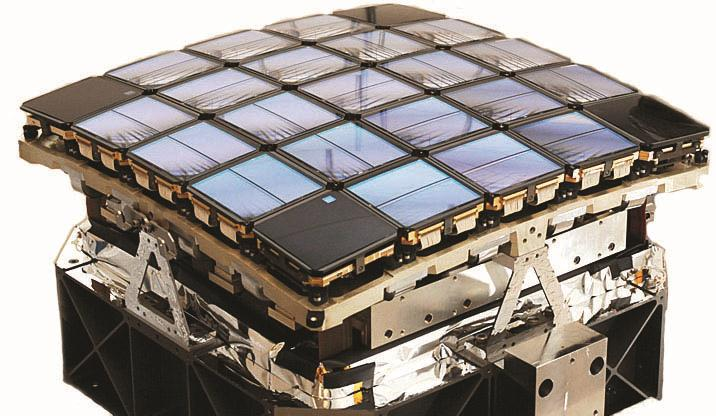
\includegraphics[width=0.3\textheight]{img/kccd.png}
	\caption{The focal plane consists of an array of 42 CCDs. Each CCD is 2.8 by 3.0 cm with 1024 by 1100 pixels. The entire focal plane contains 95 mega pixels.
mage Credits: NASA Ames and Ball Aerospace} \label{fig:kccd}
\end{center}
\end{figure}

\section{The Transit Method of Detecting Extrasolar Planets}

The Kepler spacecraft detects exoplanets using transit photometry \cite{2000ApJ...529L..45C}. If a planet orbiting a star on the plain of view and when the it moves between the detector and the star, the light that is coming from the star partially get blocked. This event is called a ``{\emph {transit}}''. For example, we can observe an occasional Venus or Mercury transit from Earth as a small black dot creeping across the Sun. During a transit, the flux we receive from the star reduce due to the transiting planet. When this happen, we say the planet transit the star, and can be detected using transit photometry. During these events, Kepler CCD collects raw data form of a sequence of stellar images, which are processed into "light-curves" tracking the brightness of a star over time. Light-curves are graphs that show the intensity of the light that observes from the star on the y-axis and the observation time on the x-axis (Figure \ref{fig:transit}). These transit data are rich with information about the planet-stellar system. The depth of the dip in the light curve and the size of the star together can be use to measure the size or the radius of the planet. The orbital period of the planet can be determined by measuring the time different between transits. Once the orbital period of the planets is known, Kepler's Third Low of planetary motion can be use to determine the average distance of the planet from its hosting star.

\begin{figure}[!h]
\begin{center}
        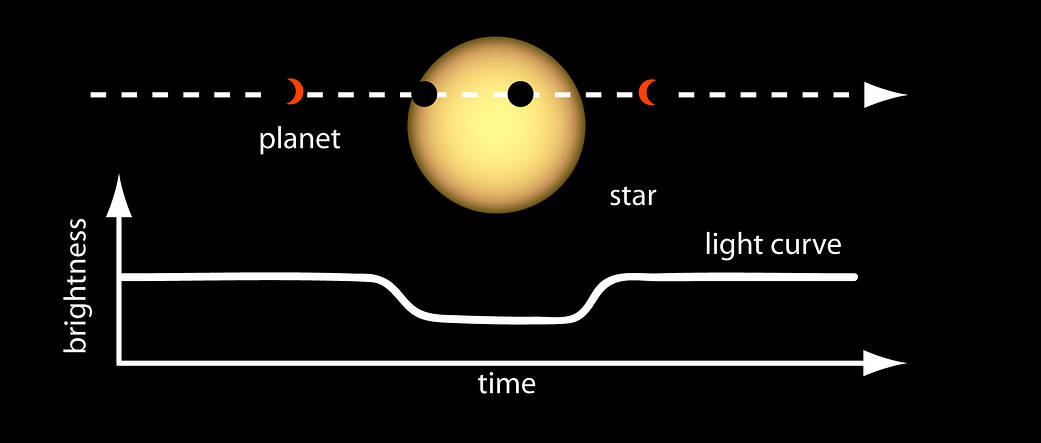
\includegraphics[width=0.7\textheight]{img/lightcurve.jpg}
        \caption{Light Curve of a Planet Transiting Its Star. Image Credit: NASA}  \label{fig:transit}
\end{center}
\end{figure}

\begin{figure}[!h]
\begin{center}
        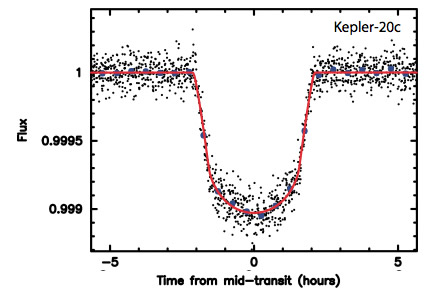
\includegraphics[width=0.6\textheight]{img/k20c.jpg}
        \caption{The light curve shown here was made from brightness data gathered by the Kepler Mission for discovery of planet Kepler-20c.
Image Credit: NASA}  \label{fig:lightcurve}
\end{center}
\end{figure}

Figure \ref{fig:lightcurve} shows the light curve made from the brightness data from Kepler Mission for the discovery of a planet named \emph{Kepler-20c}. Data clearly show the flux of the host star drop notability when the planet is in transit. This is the primary signature we are looking in the transit photometry to discover planets that are in orbits around stars. These planets create this photometric signature periodically while they are orbiting around the star. To make things more complicated, the light curves of some other objects also create similar photometric signatures: eclipsing binaries stars, certain other variable stars. During the classification stage, we need to classify these object as false positives. 


\section{Kepler Field of View (FOV)}
When it comes to where to look for exoplanets, there is a vast area in the sky we could point the spacecraft; however, there are a couple of technical requirements need to satisfy for the spacecraft to collect accurate data. The primary requirement is the field of view is always clear of the Sun and the Moon. This is preventing the Sunlight enter int to the CCD array. Kepler points away from the ecliptic, the line in the sky where the Sun, Moon, and the solar system planets traverse. Additionally, Kepler chose to look at an arm of the Milky Way galaxy that has stars similar in age and composition to our Sun and have the largest possible number of stars. The field of view region the Kepler mission is in the constellations Cygnus and Lyra, north of the visible band of the Milky Way. Figure \ref{fig:FOV2} show the Field of View superimposed over Milky Way Galaxy, Figure \ref{fig:FOV1} show the FOV relative to our Sun, Figure \ref{fig:FOV3} show the FOV relative to Cygnus. 
\begin{figure}[!h]
\begin{center}
        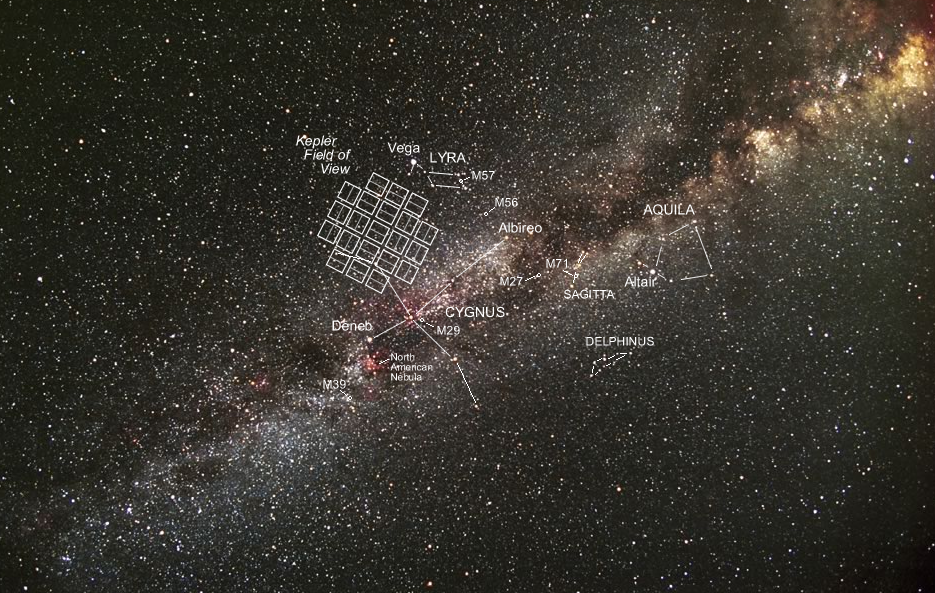
\includegraphics[width=0.55\textheight]{img/FOV2.png}
        \caption{The Kepler field of view superimposed over a photograph of the Milky Way Galaxy}  \label{fig:FOV2}
\end{center}
\end{figure}
\begin{figure}[!htb]
\minipage{0.47\textwidth}
  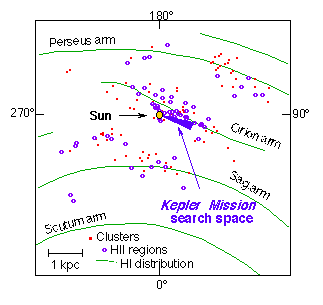
\includegraphics[width=\linewidth]{img/FOV1.png}
  \caption{Kepler FOV in extended solar neighborhood}\label{fig:FOV1}
\endminipage\hfill
\minipage{0.5\textwidth}
  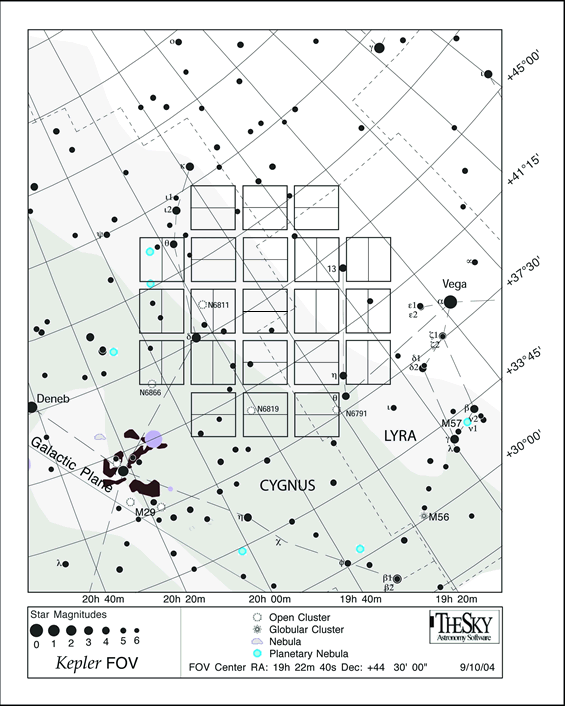
\includegraphics[width=\linewidth]{img/FOV3.png}
  \caption{Squares are 21 CCD modules.}\label{fig:FOV3}
\endminipage
\end{figure}

%\section{Kepler Data Pipleline}

\section{Kepler Pipeline}

The Kepler Pipeline \cite{2010ApJ...713L..87J} is a data reduction pipeline used for translating the Kepler raw pixel data into possible transiting planet detections. Kepler mission perform photometric observations of carefully selected stars (around 156,000) using its 115 deg$^2$ field of view (FOV) as reviewed in Borucki et el. (2010) \cite{Borucki977}
 and Koch et al. (2010)  \cite{2010ApJ...713L..79K}. The Kepler Mission Science Operations Center (SOC) at NASA Ames Research Center performs major functions on these datasets including calibrate CCD array, download data (light curves) from the spacecraft periodically, remove systematic noise \cite{2012PASP..124.1000S} and perform statistical tests to reject false positives and establish accurate statistical confidence in each detection.

\begin{figure}[!h]
\begin{center}
        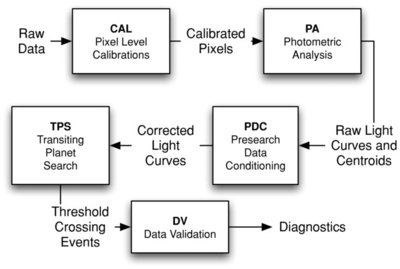
\includegraphics[width=0.5\textheight]{img/kpipeline.jpg}
        \caption{Data flow diagram for the SOC Science Pipeline. Image Credit: The American Astronomical Society}  \label{fig:kpipleline}
\end{center}
\end{figure}

Figure \ref{fig:kpipleline} show the major steps and modules of the pipeline. In particular the last two modules of the pipeline; those that identify as Threshold Crossing Events (TCEs) and their subsequent transit model fiting. TCE is a sequence of significant, periodic, planet transit-like features in the light curve of a target star. Transiting Planet Search module takes systematic error-correlated light curve for a star and seach parameter space for possible transit signatures. This module outputs a TCE or say that does not exists TCE event on the target star. This produce smaller subset of target stars what is given to the Data Validation (DV) module. DV module takes initial TCE and gaps the transit signatures from the light curve and uses the Transiting Planet Search to find additional TCEs on the same target star. This process repeats until it finds all the TCEs on given star. More details on this process explained by Mandel and Agol (2002) \cite{2002ApJ...580L.171M} and Claret and Bloemen (2011) \cite{2011yCat..35290075C}.

TPS algorithm detects transit-like features in light curves by applying noise compensating, wavelet-based matched filtering. TPS characterized the power spectral density (PSD) of the observation noise as a function of time to implement a whitening filter in the wavelet domain. The trial transit pulse is whitened and correlated against the whitened flux time series. Features with correlations above the threshold of 7.1$\sigma$ are flagged as potential threshold crossing events and subjected to additional tests in TPS to guard against false alarms.

Algorithm searches a parameter space with varying transit durations $D$ and produce a Single Event Statistics (SES) time series that is the significance of the detection of the reference transmit pulse centered at that particular time for each $D$

\begin{equation}\label{eq:ses}
	SES(t) = N(t) /\sqrt{D(t)}
\end{equation}

$\sqrt{D(t)}$, is the expected signal to noise ratio of a signal that exactly matches the template pulse and $N(t)$ is the correlated time series.



Multiple Event statistics (MES) is constructed that characterizes a significant detection in a search over varying orbital period $p$ and epochs (phase) $t_0$ by folding $N(n)$ and $D(n)$. MES  $>$ 7.1$\sigma$ may produce a TCE if it also passes additional statistical tests. SES and MES are the basis of some of the attributes used in the training set.


\section{KOI and TCE Attributes }

The Threshold Crossing Events (TCE) catalog contain a sequence of transit-like features in the flux time series of a given target star. These TCE data can download from NASA Exoplanet Archive databases \footnote{\url{http://exoplanetarchive.ipac.caltech.edu/cgi-bin/TblView/nph-tblView?app=ExoTbls&config=q1_q17_dr24_tce}}, and also the detail description of the table fields \footnote{\url{http://exoplanetarchive.ipac.caltech.edu/docs/API_tce_columns.html }} are listed as public data. Kepler Object of Interest (KOI) catalog contains object data including many attributes. The detail attributes are listed on NASA Exoplanet Archive website \footnote{\url{
http://exoplanetarchive.ipac.caltech.edu/docs/API_kepcandidate_columns.html}}, and dataset can be download from the arcive tables \footnote{\url{http://exoplanetarchive.ipac.caltech.edu/cgi-bin/TblView/nph-tblView?app=ExoTbls&config=cumulative}}. All these data cab be download as bulk using data tools available in the archive website.

%\section{Some Important Attributes}
%\label{label:important_attributes}
%There are a large number of attributes available in the KOI and TCE datasets. Out of these attributes, following attributes has significant importance in classification process according to the literature. We will be including these attributes along side with other attributes that will be determined by using Independent Component Analysis.

%\begin{itemize}
%	\item $MES_{max}$/$MES_{min}$
%	\item SNR (for all-transit model fit)
%	\item MES scaled by SES auto-correlation statistics
%	\item $\chi^{2}$ statistics for the all-transits model fit
%	\item Ratio of the planet's semi-major axis to stellar radious
%	\item The proportion of the light curve that was missing during this TCEs transit
%\end{itemize}

\section{TCE Classification Labels}

Each Threshold Crossing Event (TCE) is subject to a vetting process performed by the Kepler TCE Review Team (TCERT). During the triage (Initial) vetting stage, all TCEs are partition into two different sets: Problematic Ligh Curves that has instrumental noise and Kepler Object of Interest. KOI is a TCE that contains convincing transit-like features that do not present obvious evidence that the TCE was generated from non-transiting phenomena such as instrumental noise. These KOIs moves to next level of the vetting process performed by individuals manually inspecting light curves using detection statistics. Any indication they see the signal came from an eclipsing binary star or more complex forms of instrumental noise removed from the list. TCEs that survive this removal process are classified as Planet Candidates (PC).


We can identify three different types of classification labels in the processed dataset: Planetary Candidates (PC), Astrophysical False Positives (AFP) and non-transiting phenomena (NTP). PCs are confirmed as planets, statistically validated as planets or determined to be a planet candidate by the TCERT. AFPs are those TCEs that have been shown to be eclipsing binary stars or have shown evidence that the transiting object being detected is not located around the target tart. NTP are those TCEs that failed the initial vetting process.

%I am planning to use machine learning algorithm (Neural Network) to find a function that maps attributes produced by the Kepler Pipeline for each TCE to a classification label of PC, AFP or NTP. This classification funtion is purely based on the statistical distributions of the attributes for each TCE and the algorithm does not attempt to physically model the process of the planet transit beyond what is already present in the TCE attribute catalogs.


% \todo{Define the Problem we are solving - Classify the TCE catalog is the probme we are trying to solve}
\section{The Problem statement}

Kepler is a single instrument spacecraft that collect most contiguous and long-running photometric time series possible. Kepler observe approximately 170,000 stars simultaneously while it is operating. The fundamental objective of the Kepler mission is to detect a large number of transiting exoplanets. The ultimate goal of the primary mission was a characterize the frequency of exoplanets on diameter, orbital period and host star.  The Manual classification of the findings of Kepler object has proven very time-consuming. The new space-based, transit photometry missions such as K2 \cite{2014PASP..126..398H}, TESS \cite{2014SPIE.9143E..20R}, and PLATO 2.0 \cite{2014ExA....38..249R} also produce a large number of the dataset that demands some level of automation to do the classification. 

Using machine learning classification techniques, we can speed up the process and provide a more continuous rating of planarity candidates. There are various of machine learning classification techniques has been applied to Kepler dataset including random forests, SVM, K-mean clustering \cite{2015ApJ...800...99T, 2015ApJ...806....6M}.  In this project, we are attempting to train a Multilayered Neural Network to identify the potential planetary candidates in the Kepler dataset. 


\section{Solution Statement}

Machine learning techniques contribute a way to automate some step of exoplanet discovery. The TCE vetting process is a tedious and time-consuming (mostly a manual) process. Modern astronomical observational instruments generate a large amount of data within a short period of observational time. These observations may contain such a crucial events that need future follow-up observations using other telescopes (using other wavelengths); hence, processing these time series data and extracting meaningful information is a time sensitive process. Solution to this is to process Kepler data using machine learning algorithms to express the classification while reducing human errors. I am attempting to trained Neural Network to process the TCE catalog to automate the classification process. 


% - Explain the light curves - DONE 
% - Explain basic structure and some info about the spacecraft - DONE
% - Include some images of the field of view and spacecraft  - DONE
% \todo{Transit method - This is already Done}
% \todo{Kepler data pipeline - this is already done}
% \todo{Define the Problem we are solving - Classify the TCE catalog is the probme we are trying to solve} - DONE
% \todo{Stratergy to solve the problem - Use neural network} - Done
% \todo{Matrix that will be using - Loss function (explain the negative log likelyhood) and the confution matrix}
\chapter{Analysis}
% http://exoplanetarchive.ipac.caltech.edu/docs/API_kepcandidate_columns.html#tce_info

% % Start with this 
% https://arxiv.org/pdf/1201.1048.pdf (Transiting Planet Search section)
% also plot some field and explain the fileds in details (in this paper and also in the main paper)

% TCE http://exoplanetarchive.ipac.caltech.edu/docs/TableColumnDescriptors.html#targets

% http://exoplanetarchive.ipac.caltech.edu/docs/tce_releasenotes_q1q12.pdf


	
% If a dataset is present, 
	% features 
	% calculated statistics relevant to the problem 
	% sampling of the data.

A Threshold-Crossing Events (TCE) are built using flux time series that has a sequence of transit-like features. The flux time series of a target star that resembles the signature of transiting planet with a high degree of confidence passed on for further analysis. Each TCE identified by a Kepler ID (KID). In the case of a star that holds multiple planets may have a many TCEs. Figure \ref{fig:TCE_lightcurves} show examples of two classes of TCEs. In the top plot is the flux time series for a true transiting planet candidate, with transit-like features of comparable depth. In the bottom plot is a flux time series containing a single very large feature and a bump that is slight above the noise floor; the Kepler pipeline identifies this flux time series as containing a
transit signature despite the fact that it is just the artifact.
 


\begin{figure}[!h]
\begin{center}
        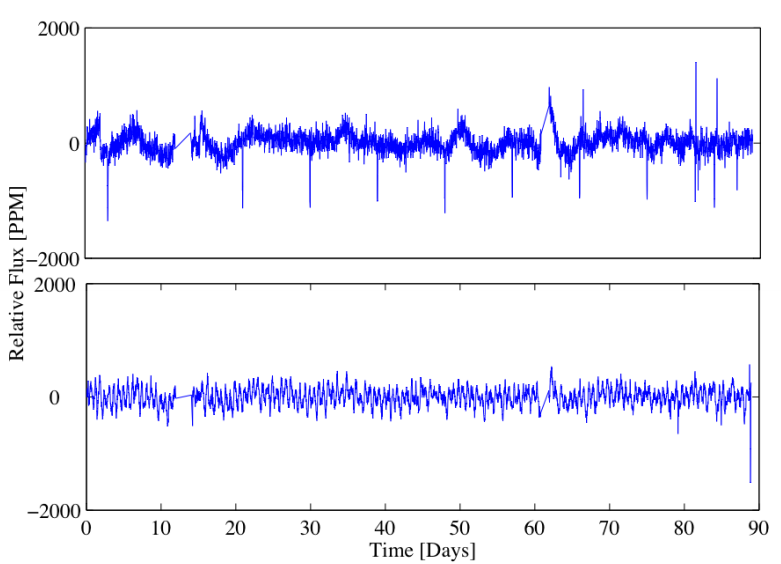
\includegraphics[width=0.7\textheight]{img/TCE_lightcurves.png}
        \caption{Two examples of light curves which produce TCEs. \emph{Top}: a planet
candidate, with multiple transit-like features of comparable depth. \emph{Bottom}: a spurious candidate, with a
single large feature at the end of the light curve and a small bump at 79 days that are combined and
interpreted as a TCE.}  \label{fig:TCE_lightcurves}
\end{center}
\end{figure}


\section{Threshold Crossing Event Catalog}

\begin{figure}[!h]
\begin{center}
        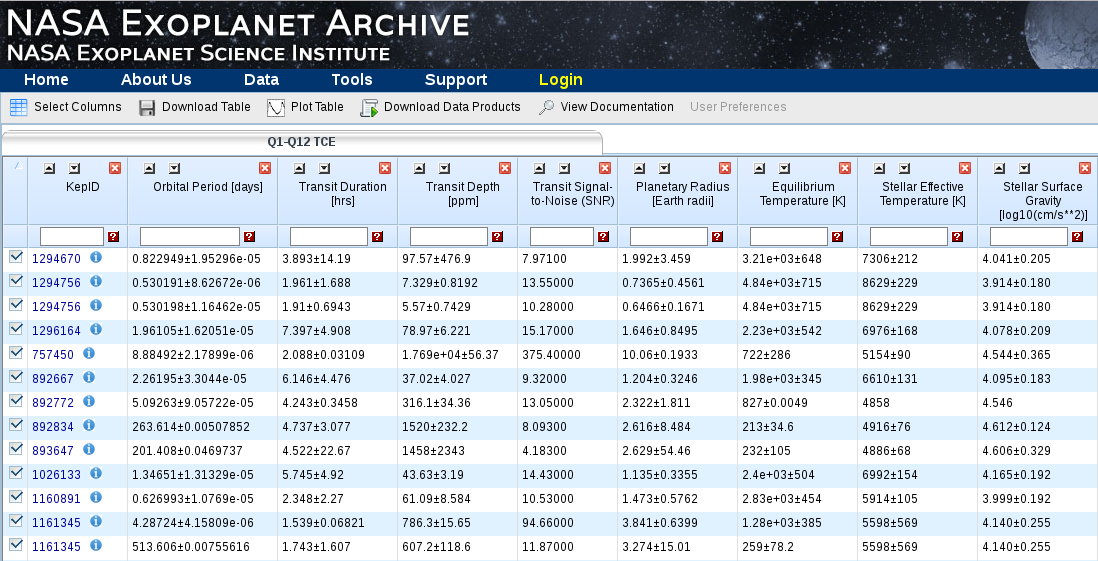
\includegraphics[width=0.8\textheight]{img/TCECatalog.png}
        \caption{Threshold Crossing Event Catalog:  \url{http://exoplanetarchive.ipac.caltech.edu/cgi-bin/TblView/nph-tblView?app=ExoTbls&config=q1_q12_tce}}  \label{fig:tcecatalog}
\end{center}
\end{figure}

Figure \ref{fig:tcecatalog} show a sample of TCE datalog from Exoplanet Archive from  NASA Exoplanet Science Institute. This is an interactive table that has exoplanet archive including information provided by the original sources. Each row that has unique KeplerID is a TCE. In Figure \ref{fig:tcecatalog} show only a few columns out of many. Each column is an observed or a computed data point that related to the given TCE. Using the upper left hand "Select Column" menu, we can select any fields to appear on the table. By hovering over a KeplerID, you can explore more data that is belong to this particular TCE (show in Figure \ref{fig:tcecatalogdetail}). Kepler target overview page show more complete stellar parameters including stellar 2MASS images. Kepler TCE Overview page shows in-depth details of the TCE, this includes Kepler data validation reports and Kepler Planet Detection Metrics and time series data including various downloading options. We can download all the time series data from these catalogs. 

\begin{figure}[!h]
\begin{center}
        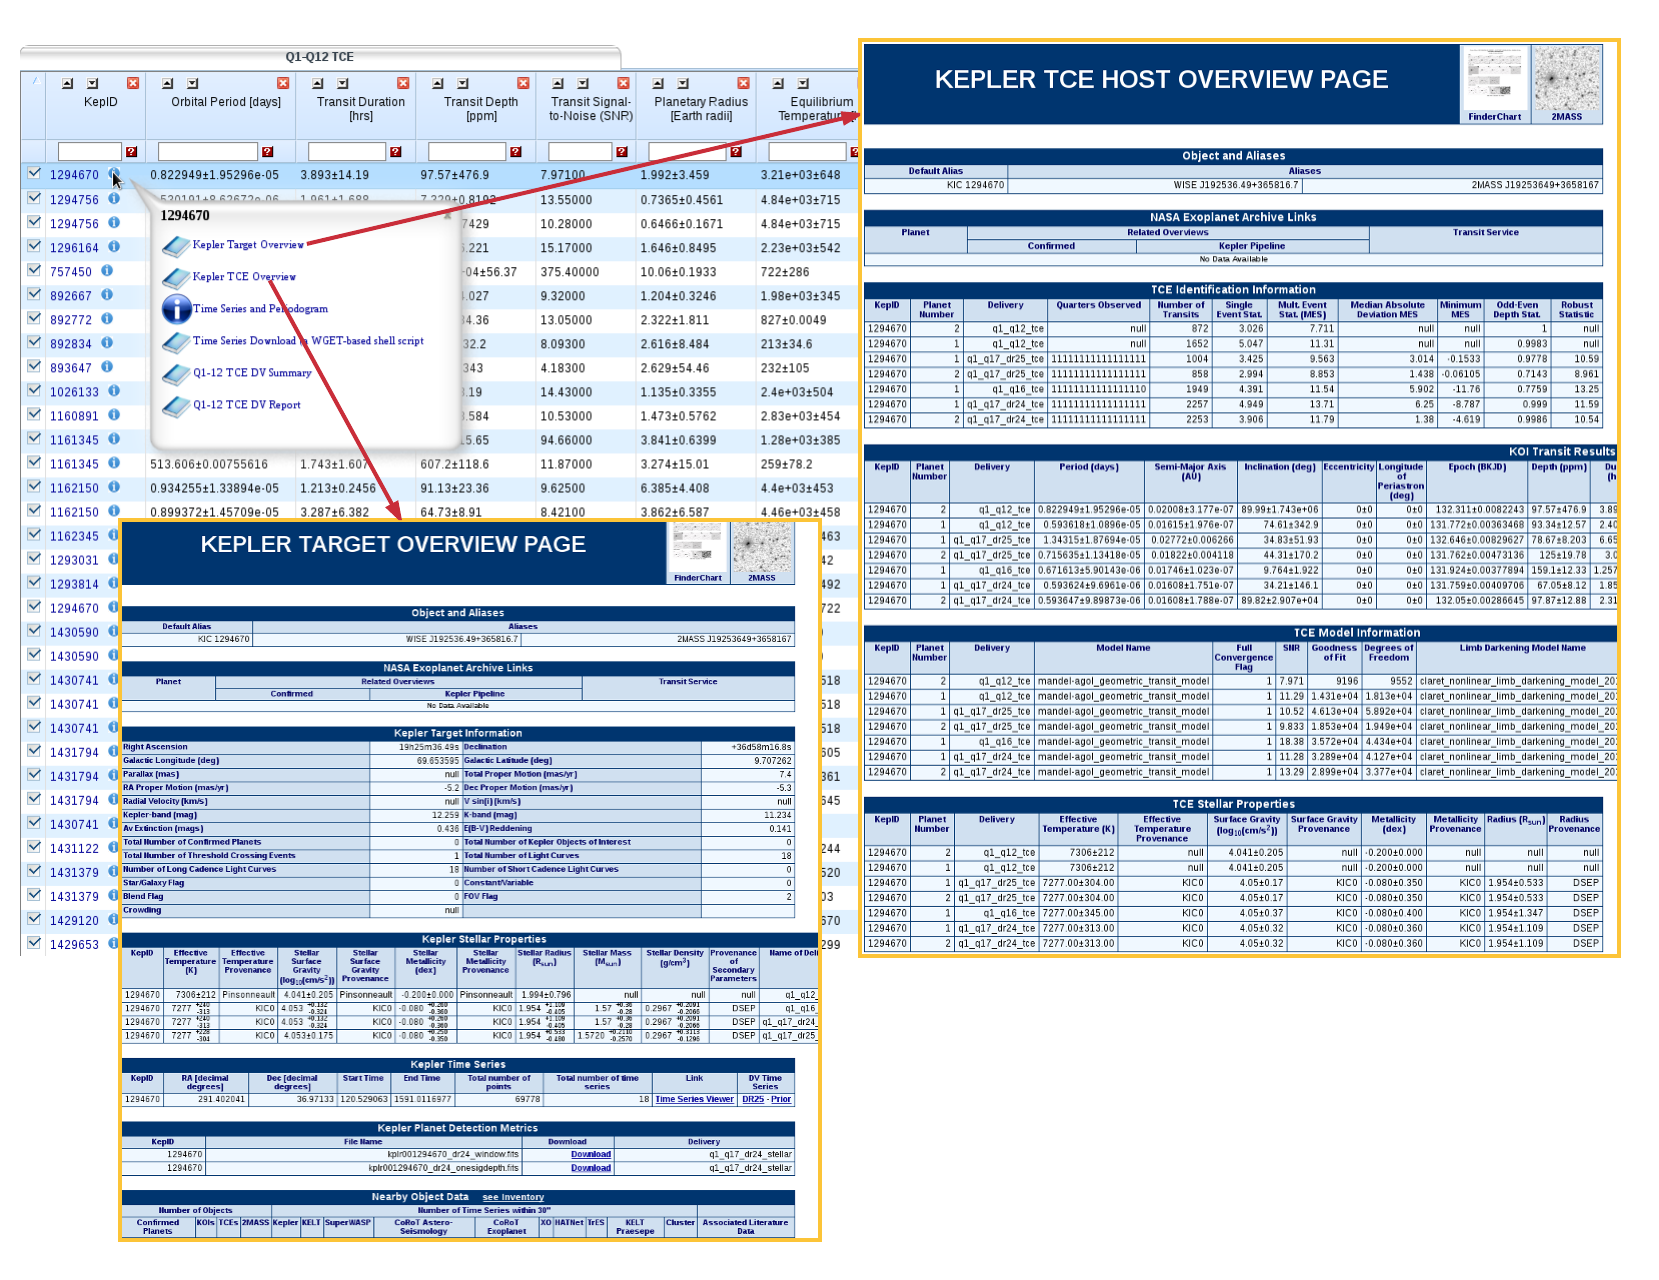
\includegraphics[width=0.8\textheight]{img/tceoptions.png}
        \caption{Threshold Crossing Event Catalog Details}  \label{fig:tcecatalogdetail}
\end{center}
\end{figure}

\section{TCE Attributes}
\label{label:tce_attributes}

Initial TCE attribute set contains 237 attributes that are based on the wavelet matched filter use by TPS, transit model fitting, difference image centroids, and some additional tests. Each of these attributes has different strength of prediction values. The importance of these attributes is selected using historical literature on attributes and performing a Principal Component Analysis. We discuss some of the most important attributes in this section.

%% Transit fit parameters
\subsection{Transit Fit Parameters}

This paper presents exact analytic formulate for the eclipse of a star described by quadratic or nonlinear limb darkening. The Kepler Project derives transit parameters from best-fit parameters produced by this analytic formula. Some of the transit parameters are calculated directly; others are derived from the best-fit parameters. Limb-darkening coefficients are fixed and pre-calculated from host stellar properties.  


\subsubsection{Ratio between planet radius and stellar radius (\emph{tce\_ror})}
This attribute is calculated using planet radius divided by its hosting the stellar radius. Both planet and stellar radius are in Eath-radii units. Plot \ref{plot:planet_star_radius_ratio} show the histogram of the \emph{tce\_ror} attribute in the TCE catalog (x-axis is in log scale and y-axis is in linear)

\begin{figure}[!h]
\begin{center}
        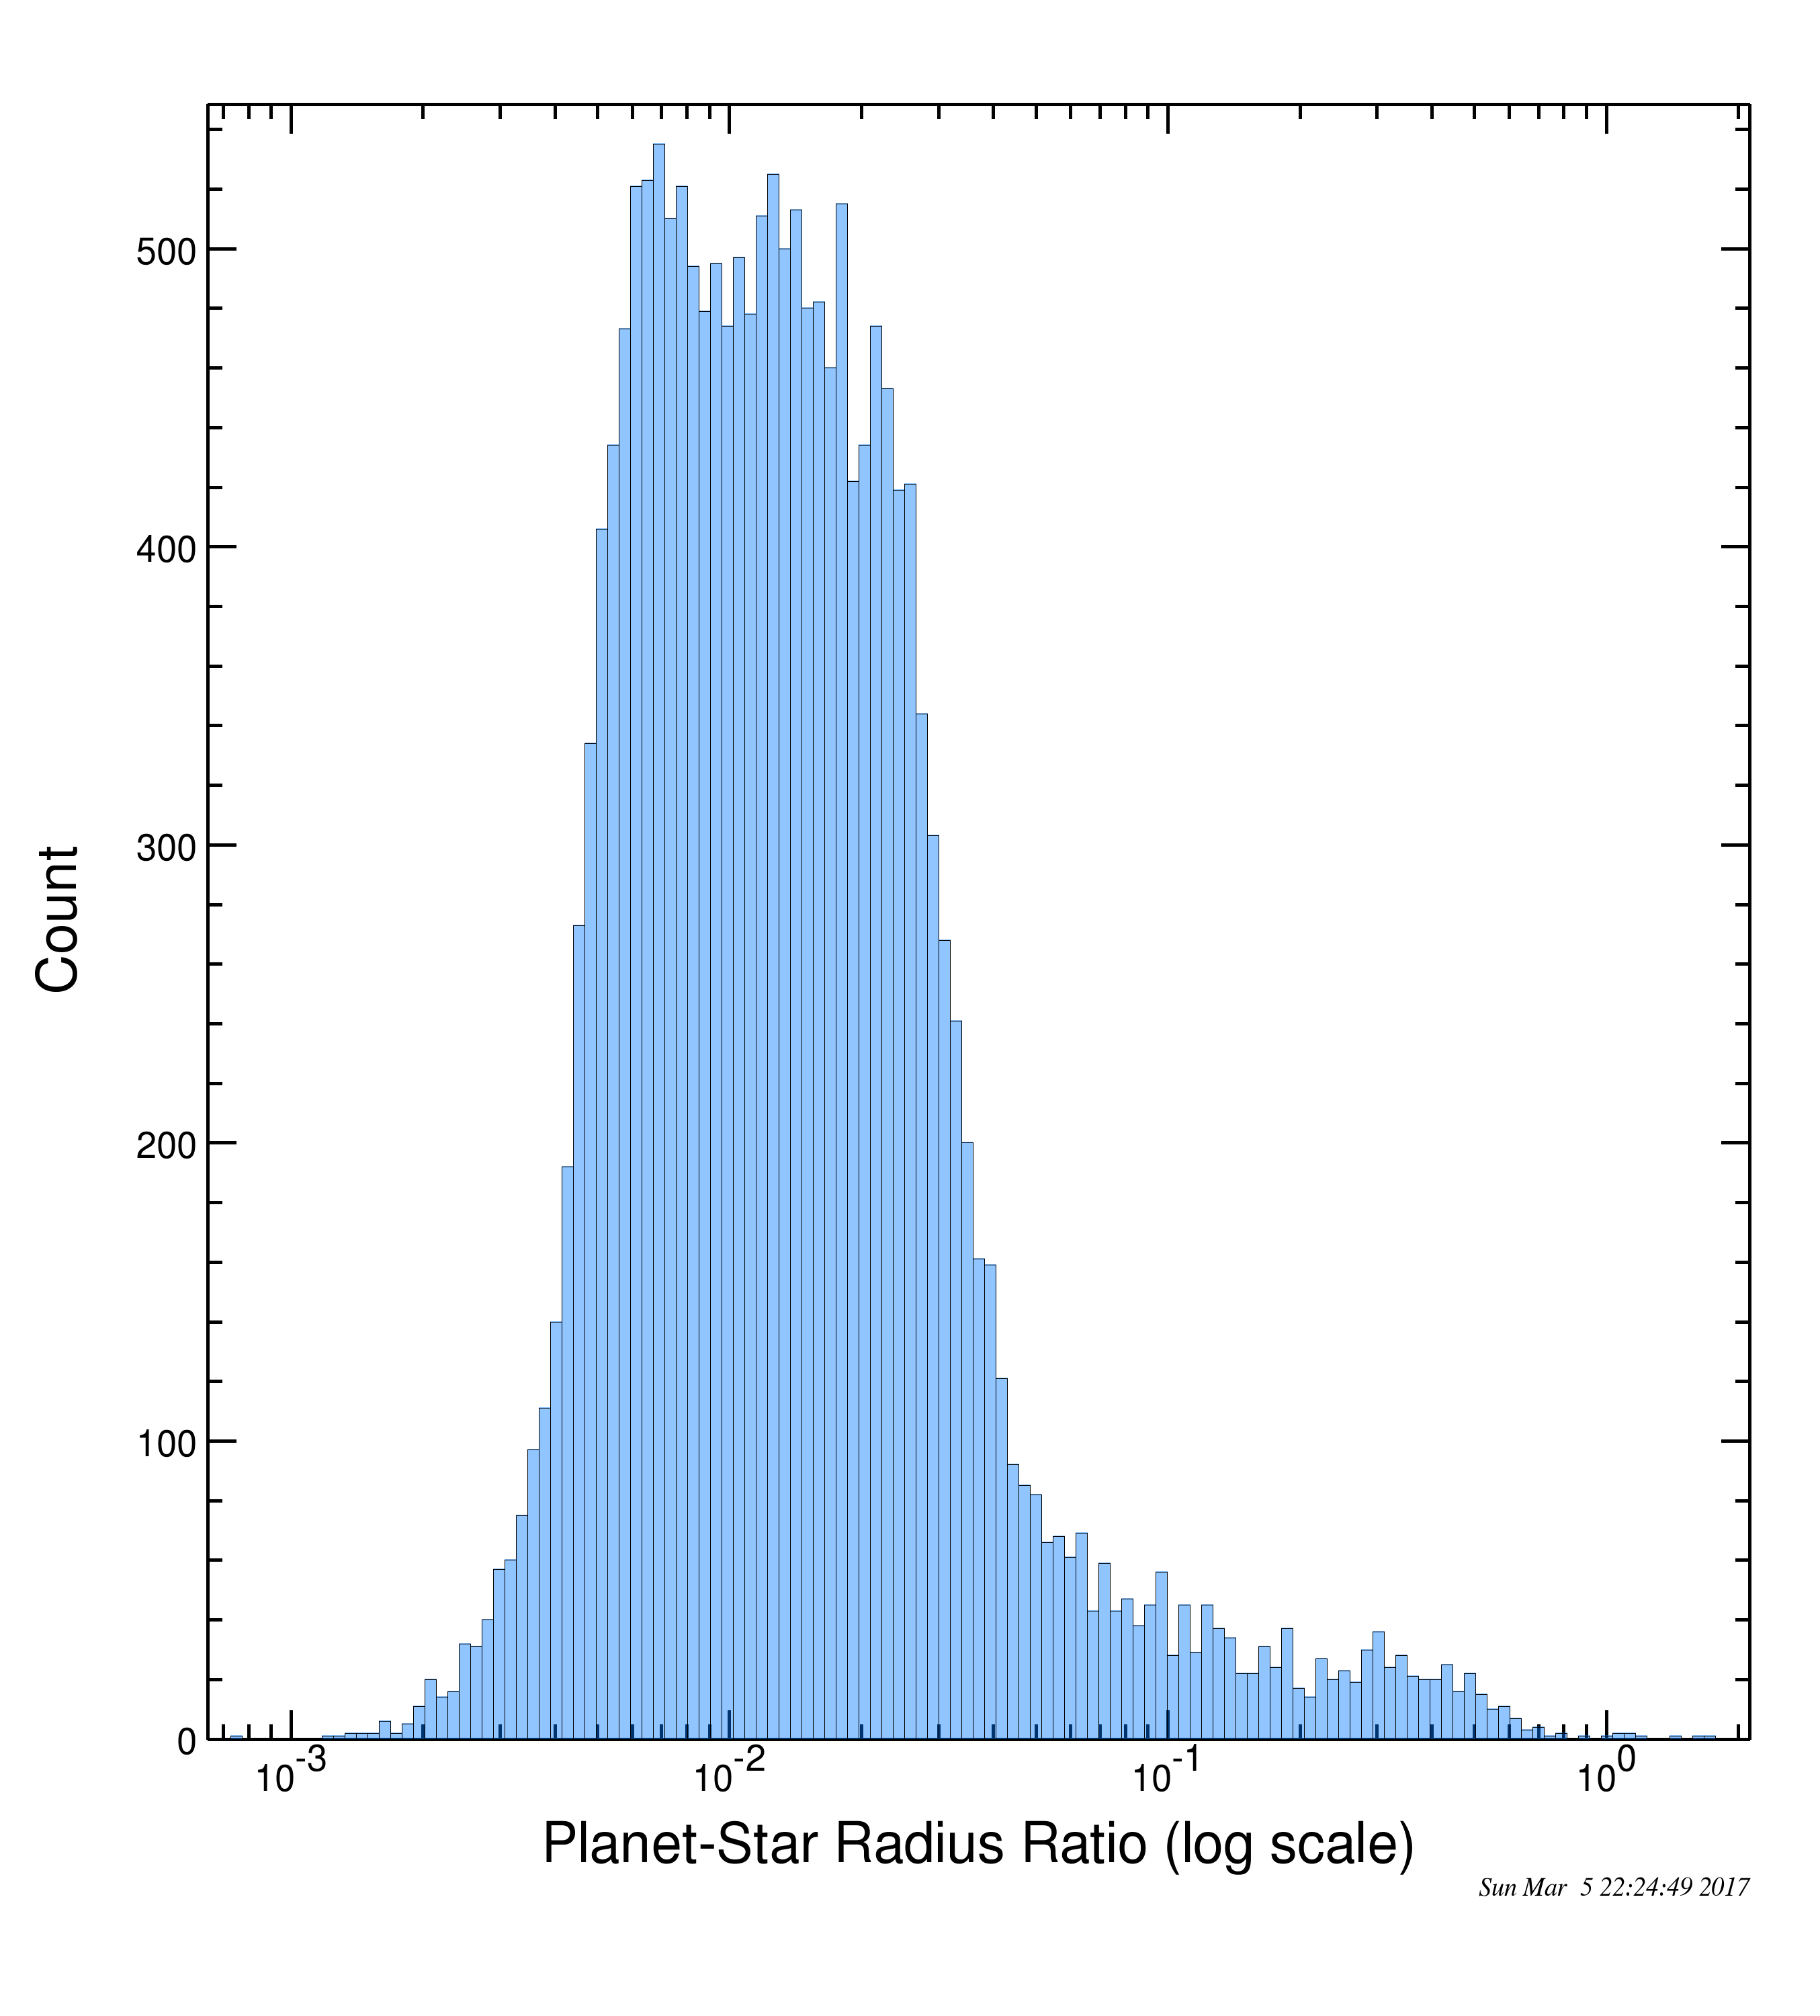
\includegraphics[width=0.5\textheight]{img/planet_star_radius_ratio.png}
        \caption{Ratio between planet radius and stellar radios}  \label{plot:planet_star_radius_ratio}
\end{center}
\end{figure}

\subsubsection{Transit Duration (\emph{tce\_duration)}}
Transit Duration is the duration of the observed transits. Duration is measured from the first contact between the planet and star until the last contact. The duration is measured by hours. The plot \ref{plot:transitduration} show the distribution of the transit duration of the TCE catalog. We can observe the most of the transit are fall under 10-hour duration.

\begin{figure}[!h]
\begin{center}
        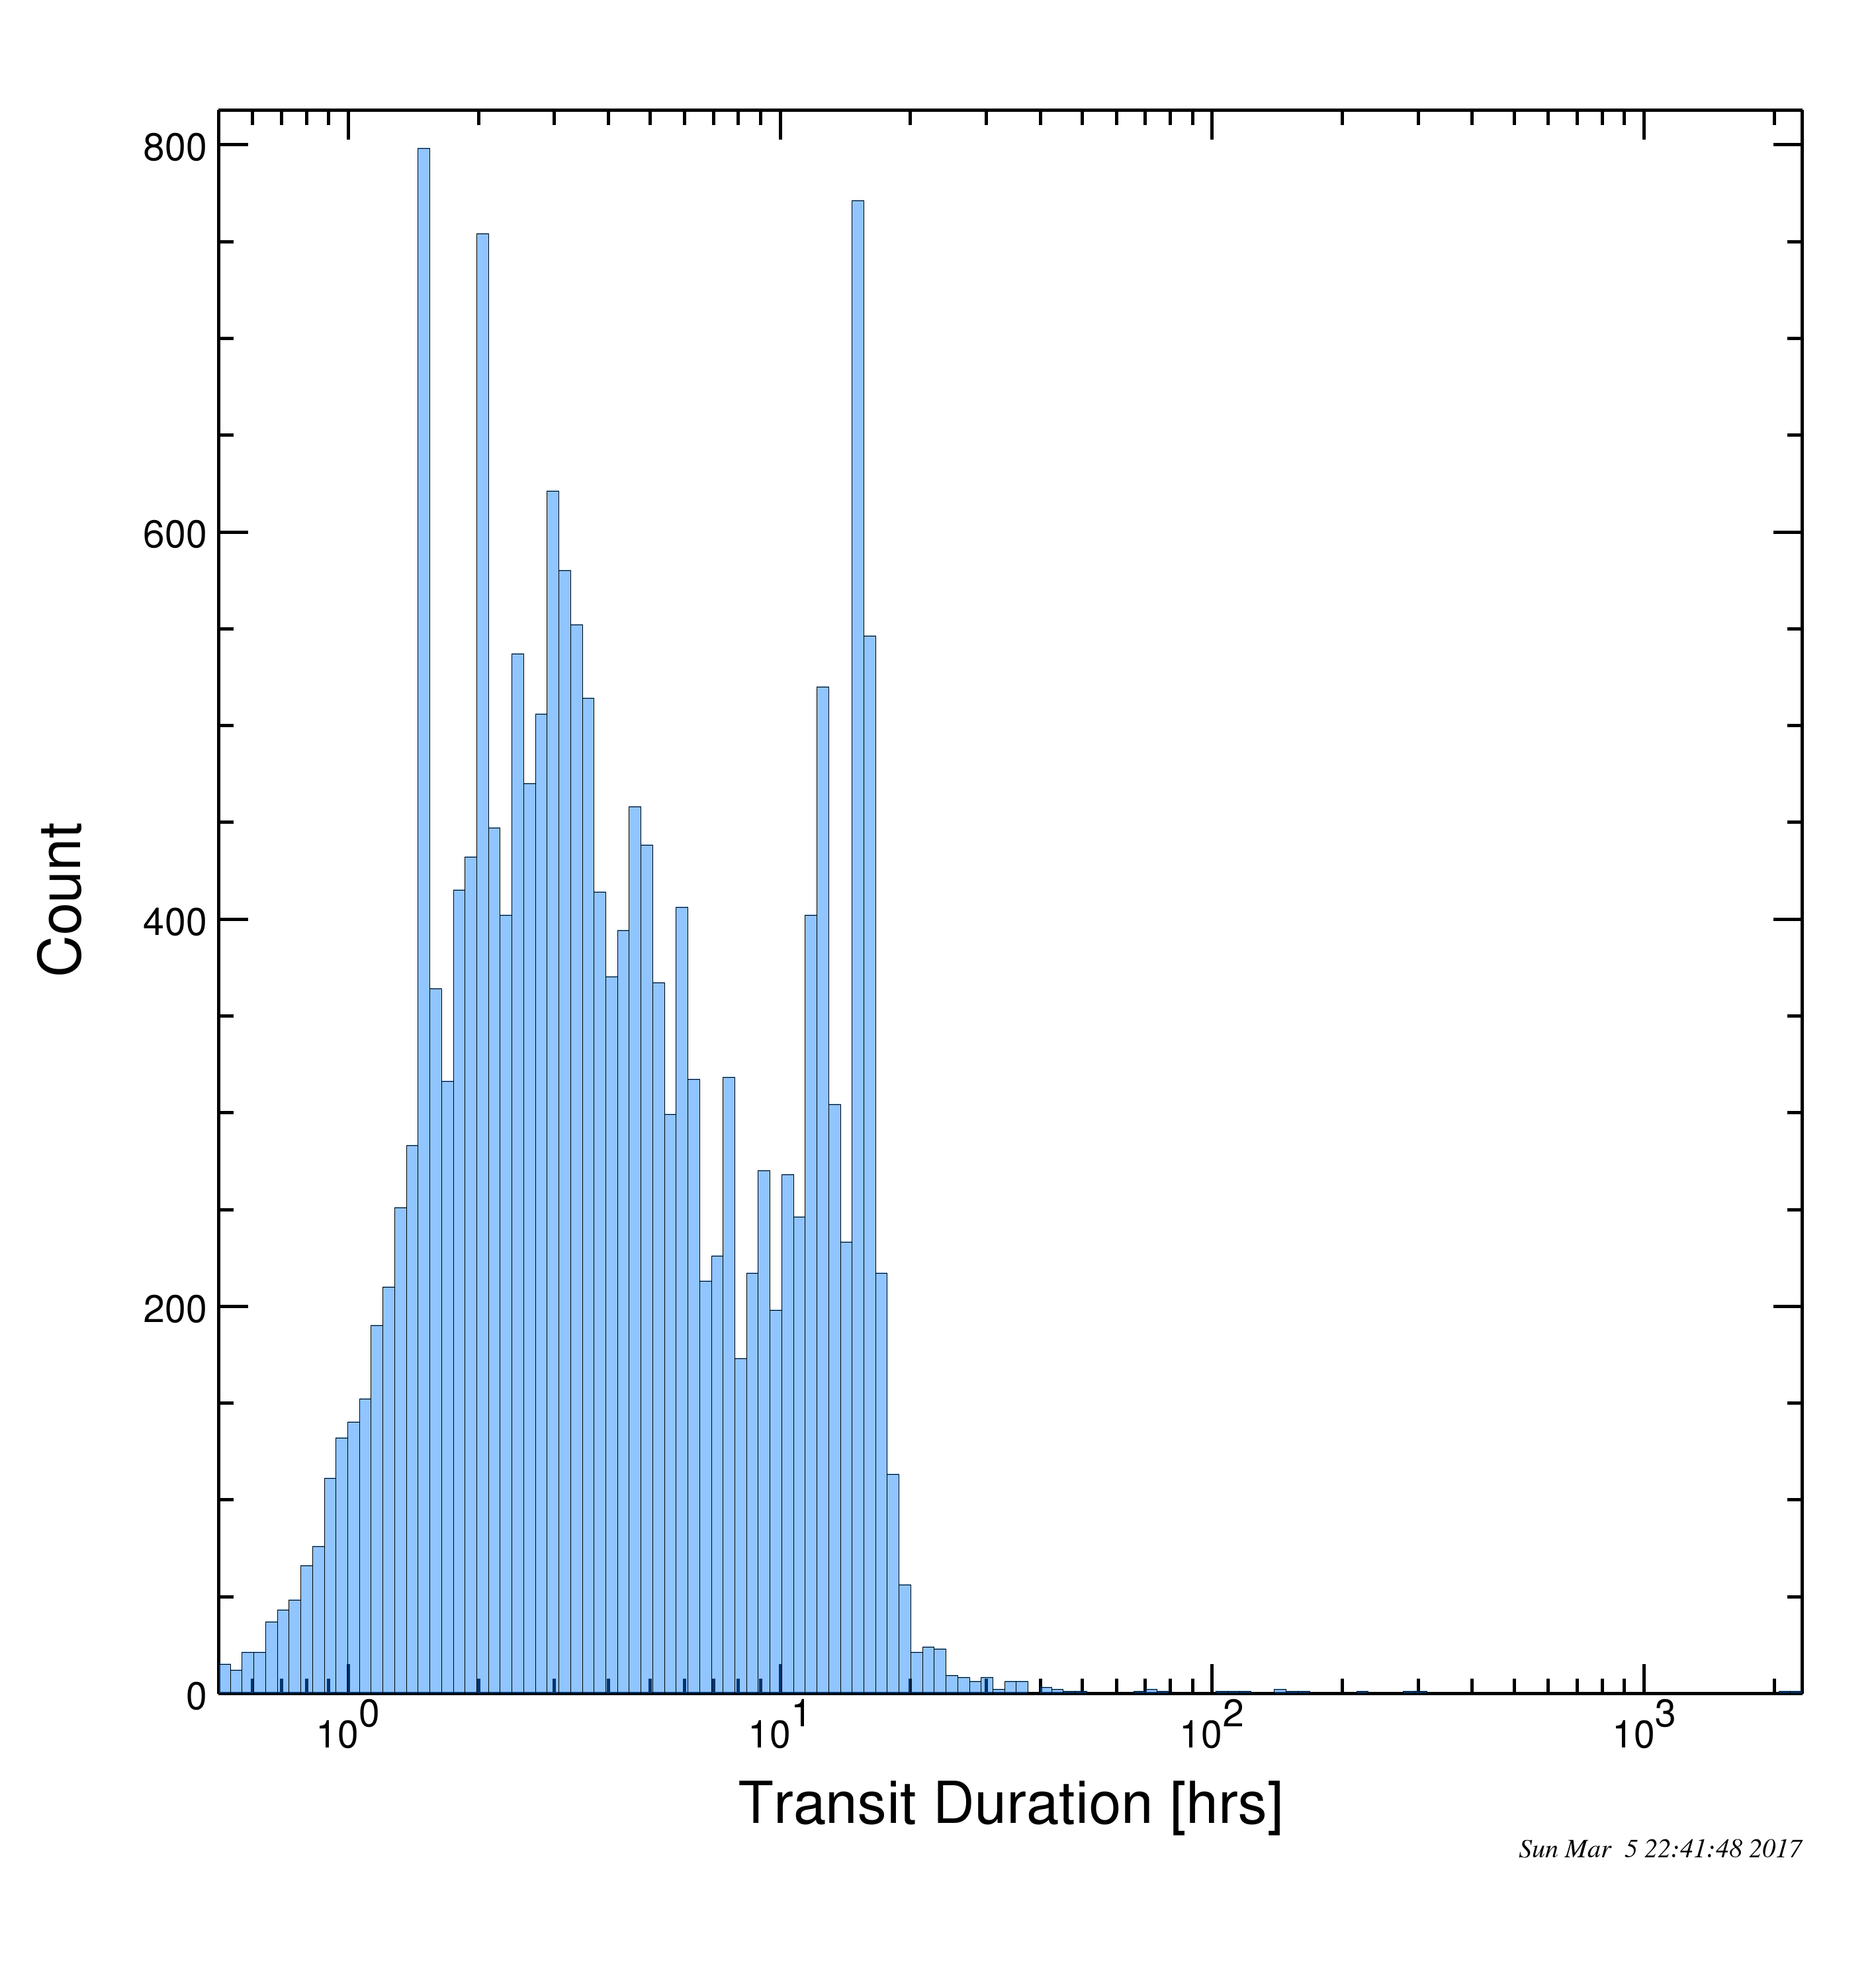
\includegraphics[width=0.5\textheight]{img/transitduration.png}
        \caption{Transit Duration}  \label{plot:transitduration}
\end{center}
\end{figure}

\subsubsection{Impact Parameter(\emph{tce\_impact})}
Impact Parameter is the sky-projected distance between the center of the stellar disc and the center of the planet disc at conjunction, normalized by the stellar radius.

\subsubsection{Transit SNR (\emph{tce\_model\_snr})}
Transit depth normalized by the mean uncertainty in the flux during the transits. Plot \ref{plot:transitsnr} show the distribution of the SNR. 

\begin{figure}[!h]
\begin{center}
        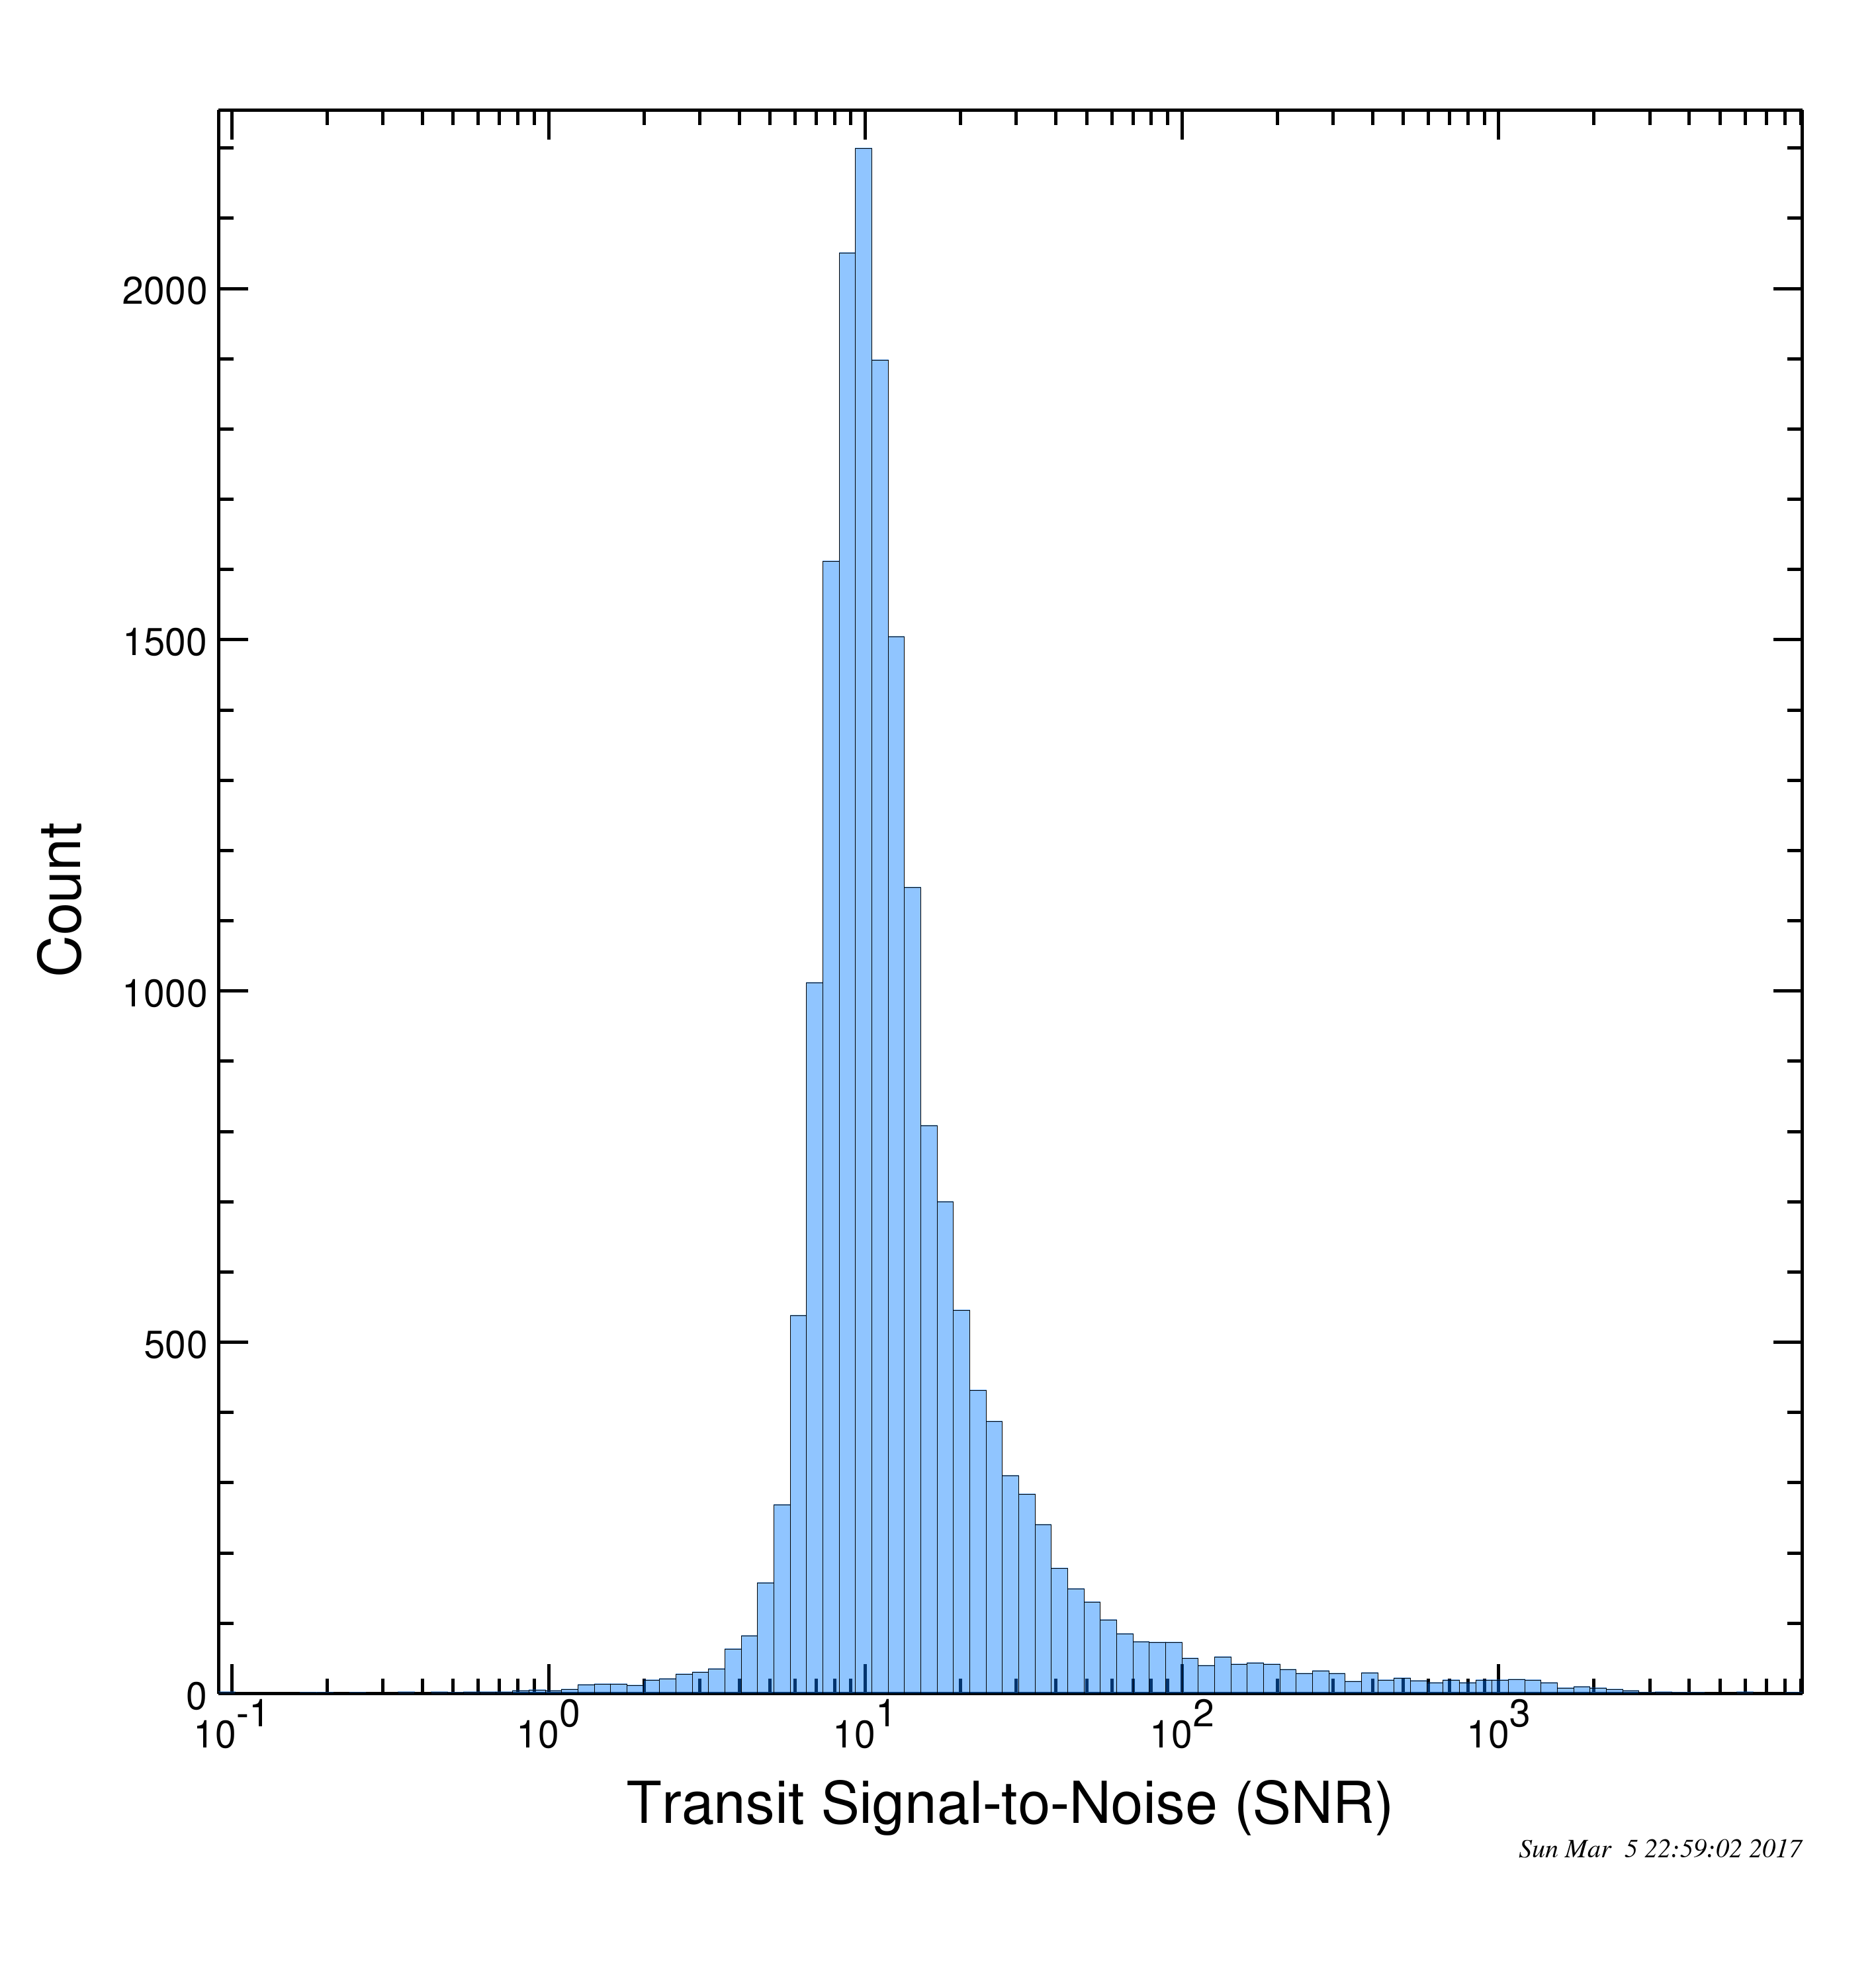
\includegraphics[width=0.5\textheight]{img/transitsnr.png}
        \caption{Transit SNR}  \label{plot:transitsnr}
\end{center}
\end{figure}

%% Stellar Parameters 
\subsection{Stellar Parameters}
Best-fit transit parameters are normalized to the size of the host star. The size of the hosting star is determined by its radius. Physical planet parameters may be derived by scaling to the star's size and temperature. Stellar effective temperature, surface gravity, metallicity, radius, mass, and age should comprise a consistent set. This section describe and visualize some of the stellar parameters from the TCE catalog.

\subsubsection{Stellar Effective Temperature (K) (\emph{tce\_steff})}
Plot \ref{plot:stellartemp} show the photospheric temperature of the stars in the TCE catalog. Kepler mission target sun-like stars and the photospheric temperature of the sun is 5,775 K. If we plot the sun on the \ref{plot:stellartemp}, it will fall close to the apparently large number count that shows on the plot. This plot \ref{plot:stellartemp} show the TCE catalog stellar temperatures are falling between 3000K and 17000K 


\begin{figure}[!h]
\begin{center}
        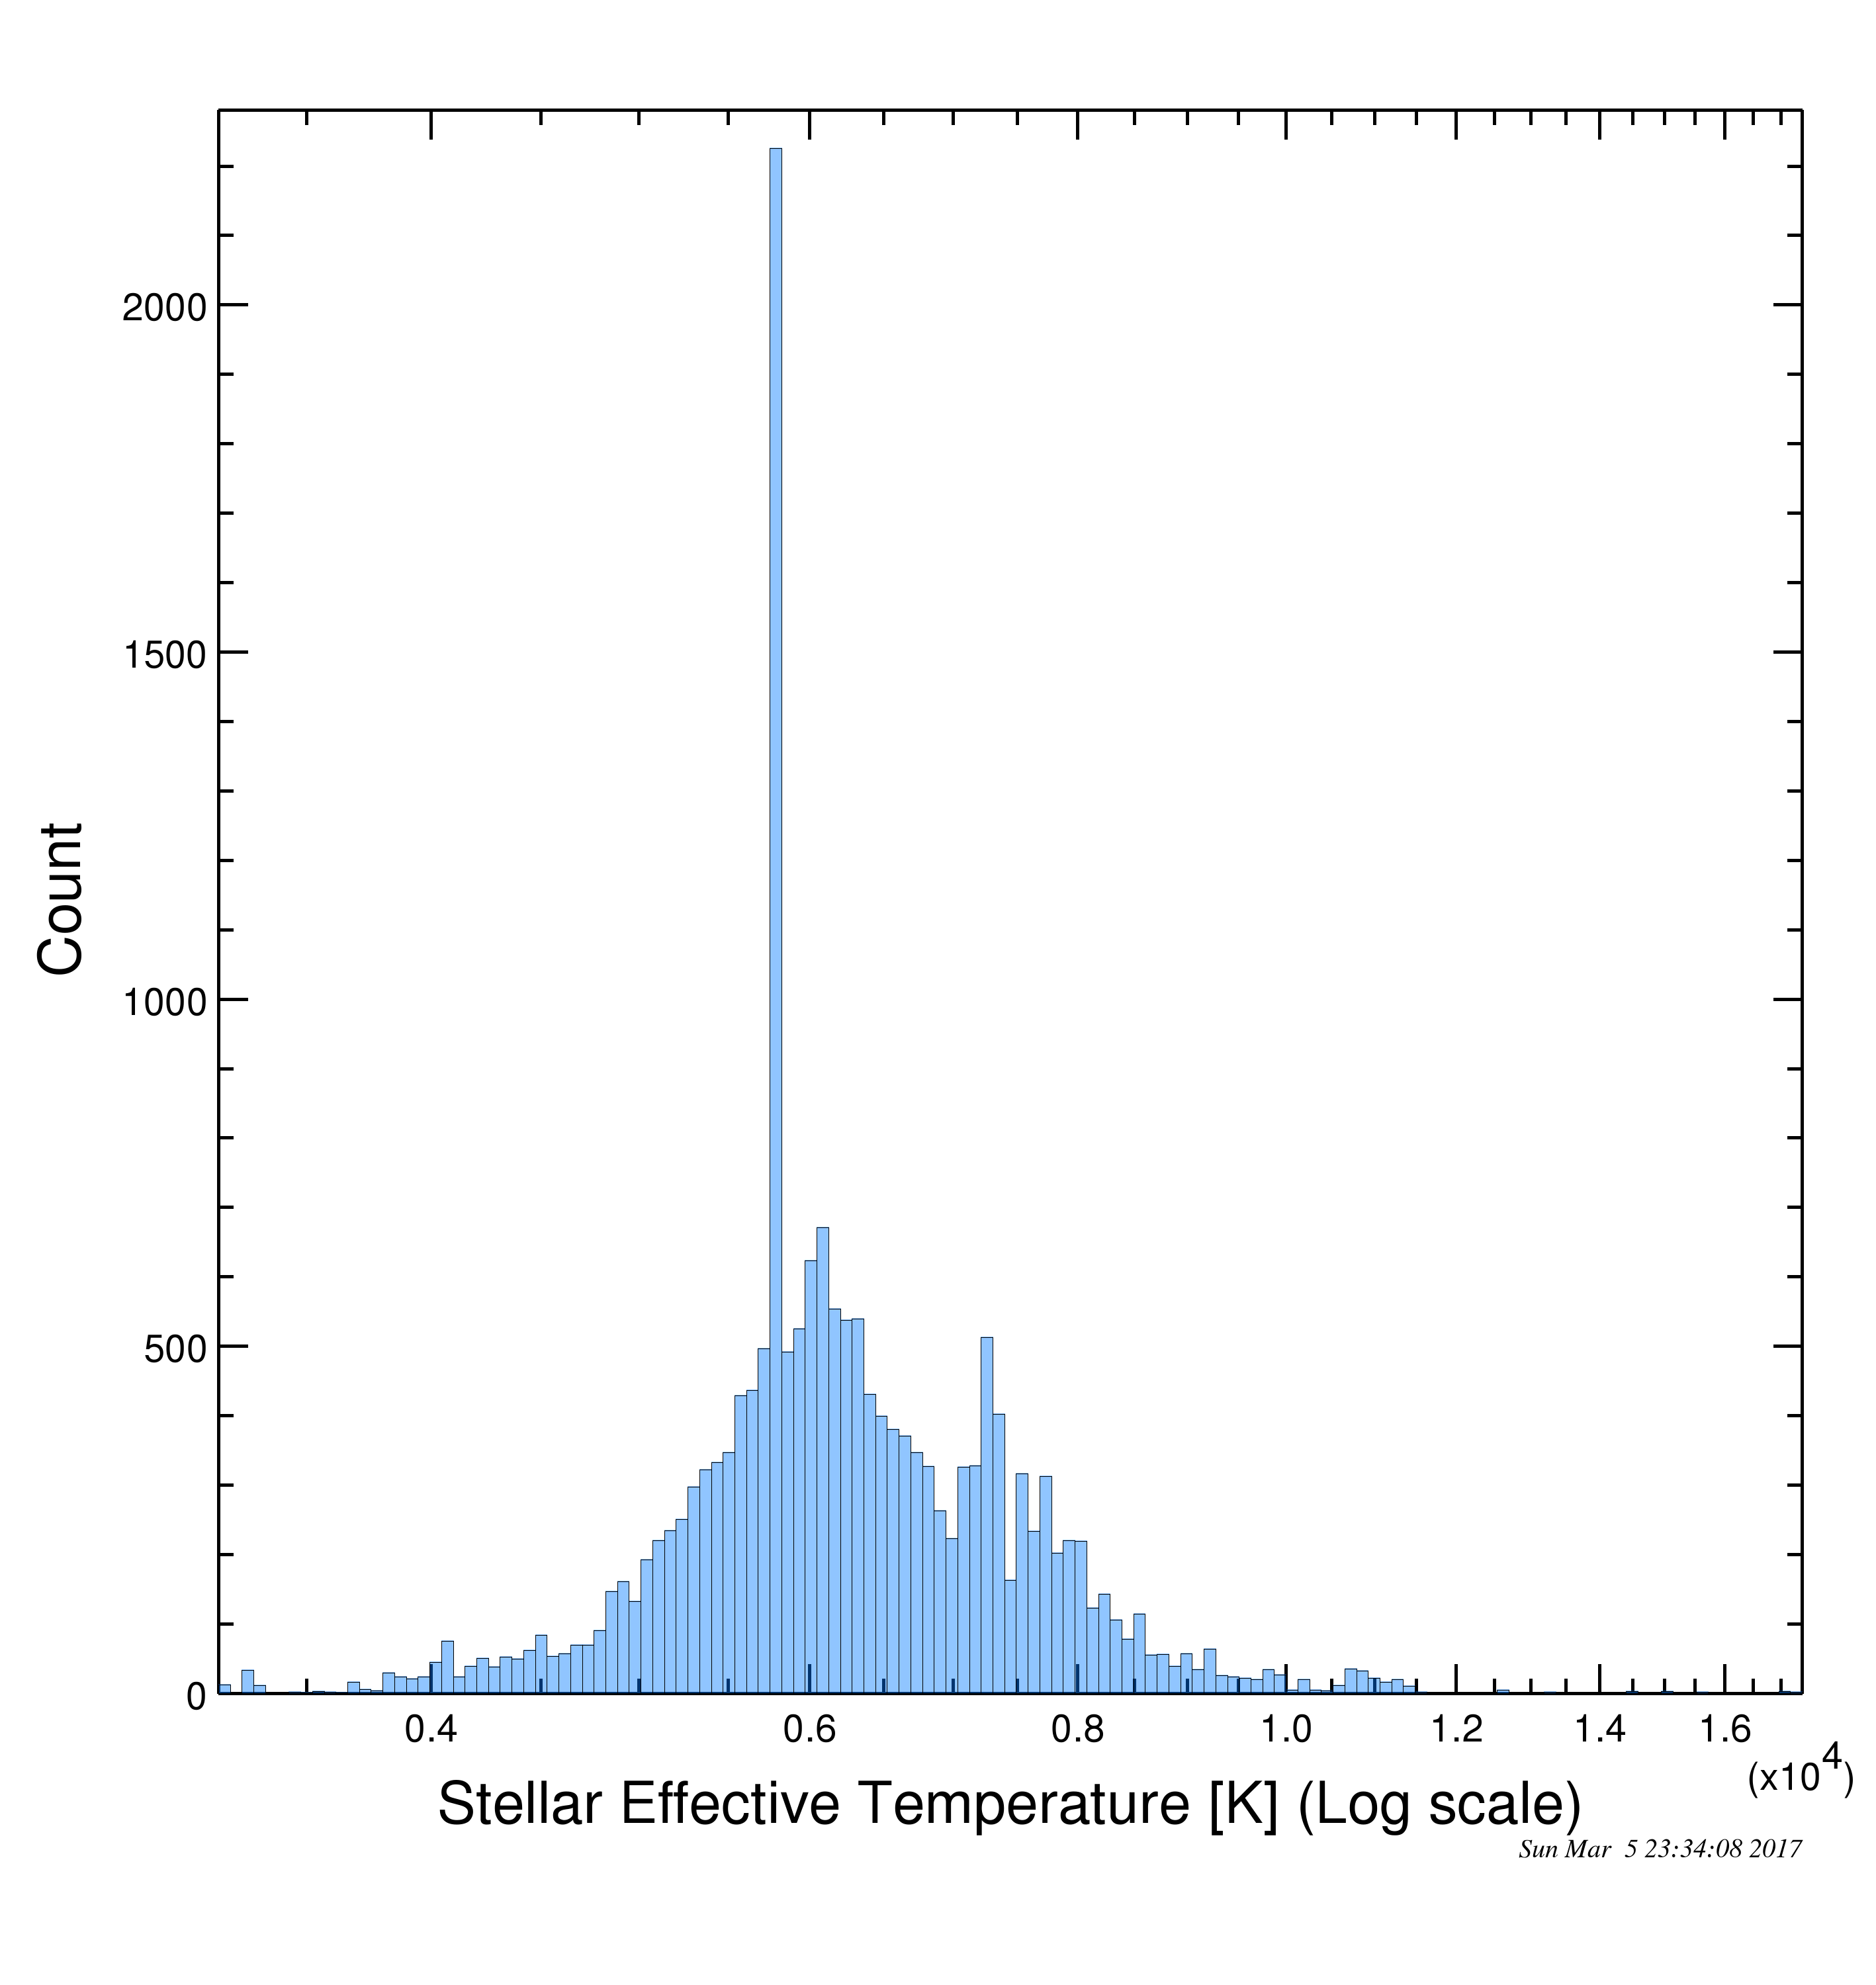
\includegraphics[width=0.5\textheight]{img/stellartemp.png}
        \caption{Stellar Effective Temperature (K)}  \label{plot:stellartemp}
\end{center}
\end{figure}

\subsubsection{Stellar Surface Gravity (\emph{tce\_slogg})}
The base-10 logarithm of the acceleration due to gravity at the surface of the star. The surface gravity of our sun is 274.0 cm/$s^{2}$ (4.44 log10(cm/$s^{2}$)). Plot \ref{plot:stellargravity} show the distribution of the TCE catalog stellar surface gravity. 

\begin{figure}[!h]
\begin{center}
        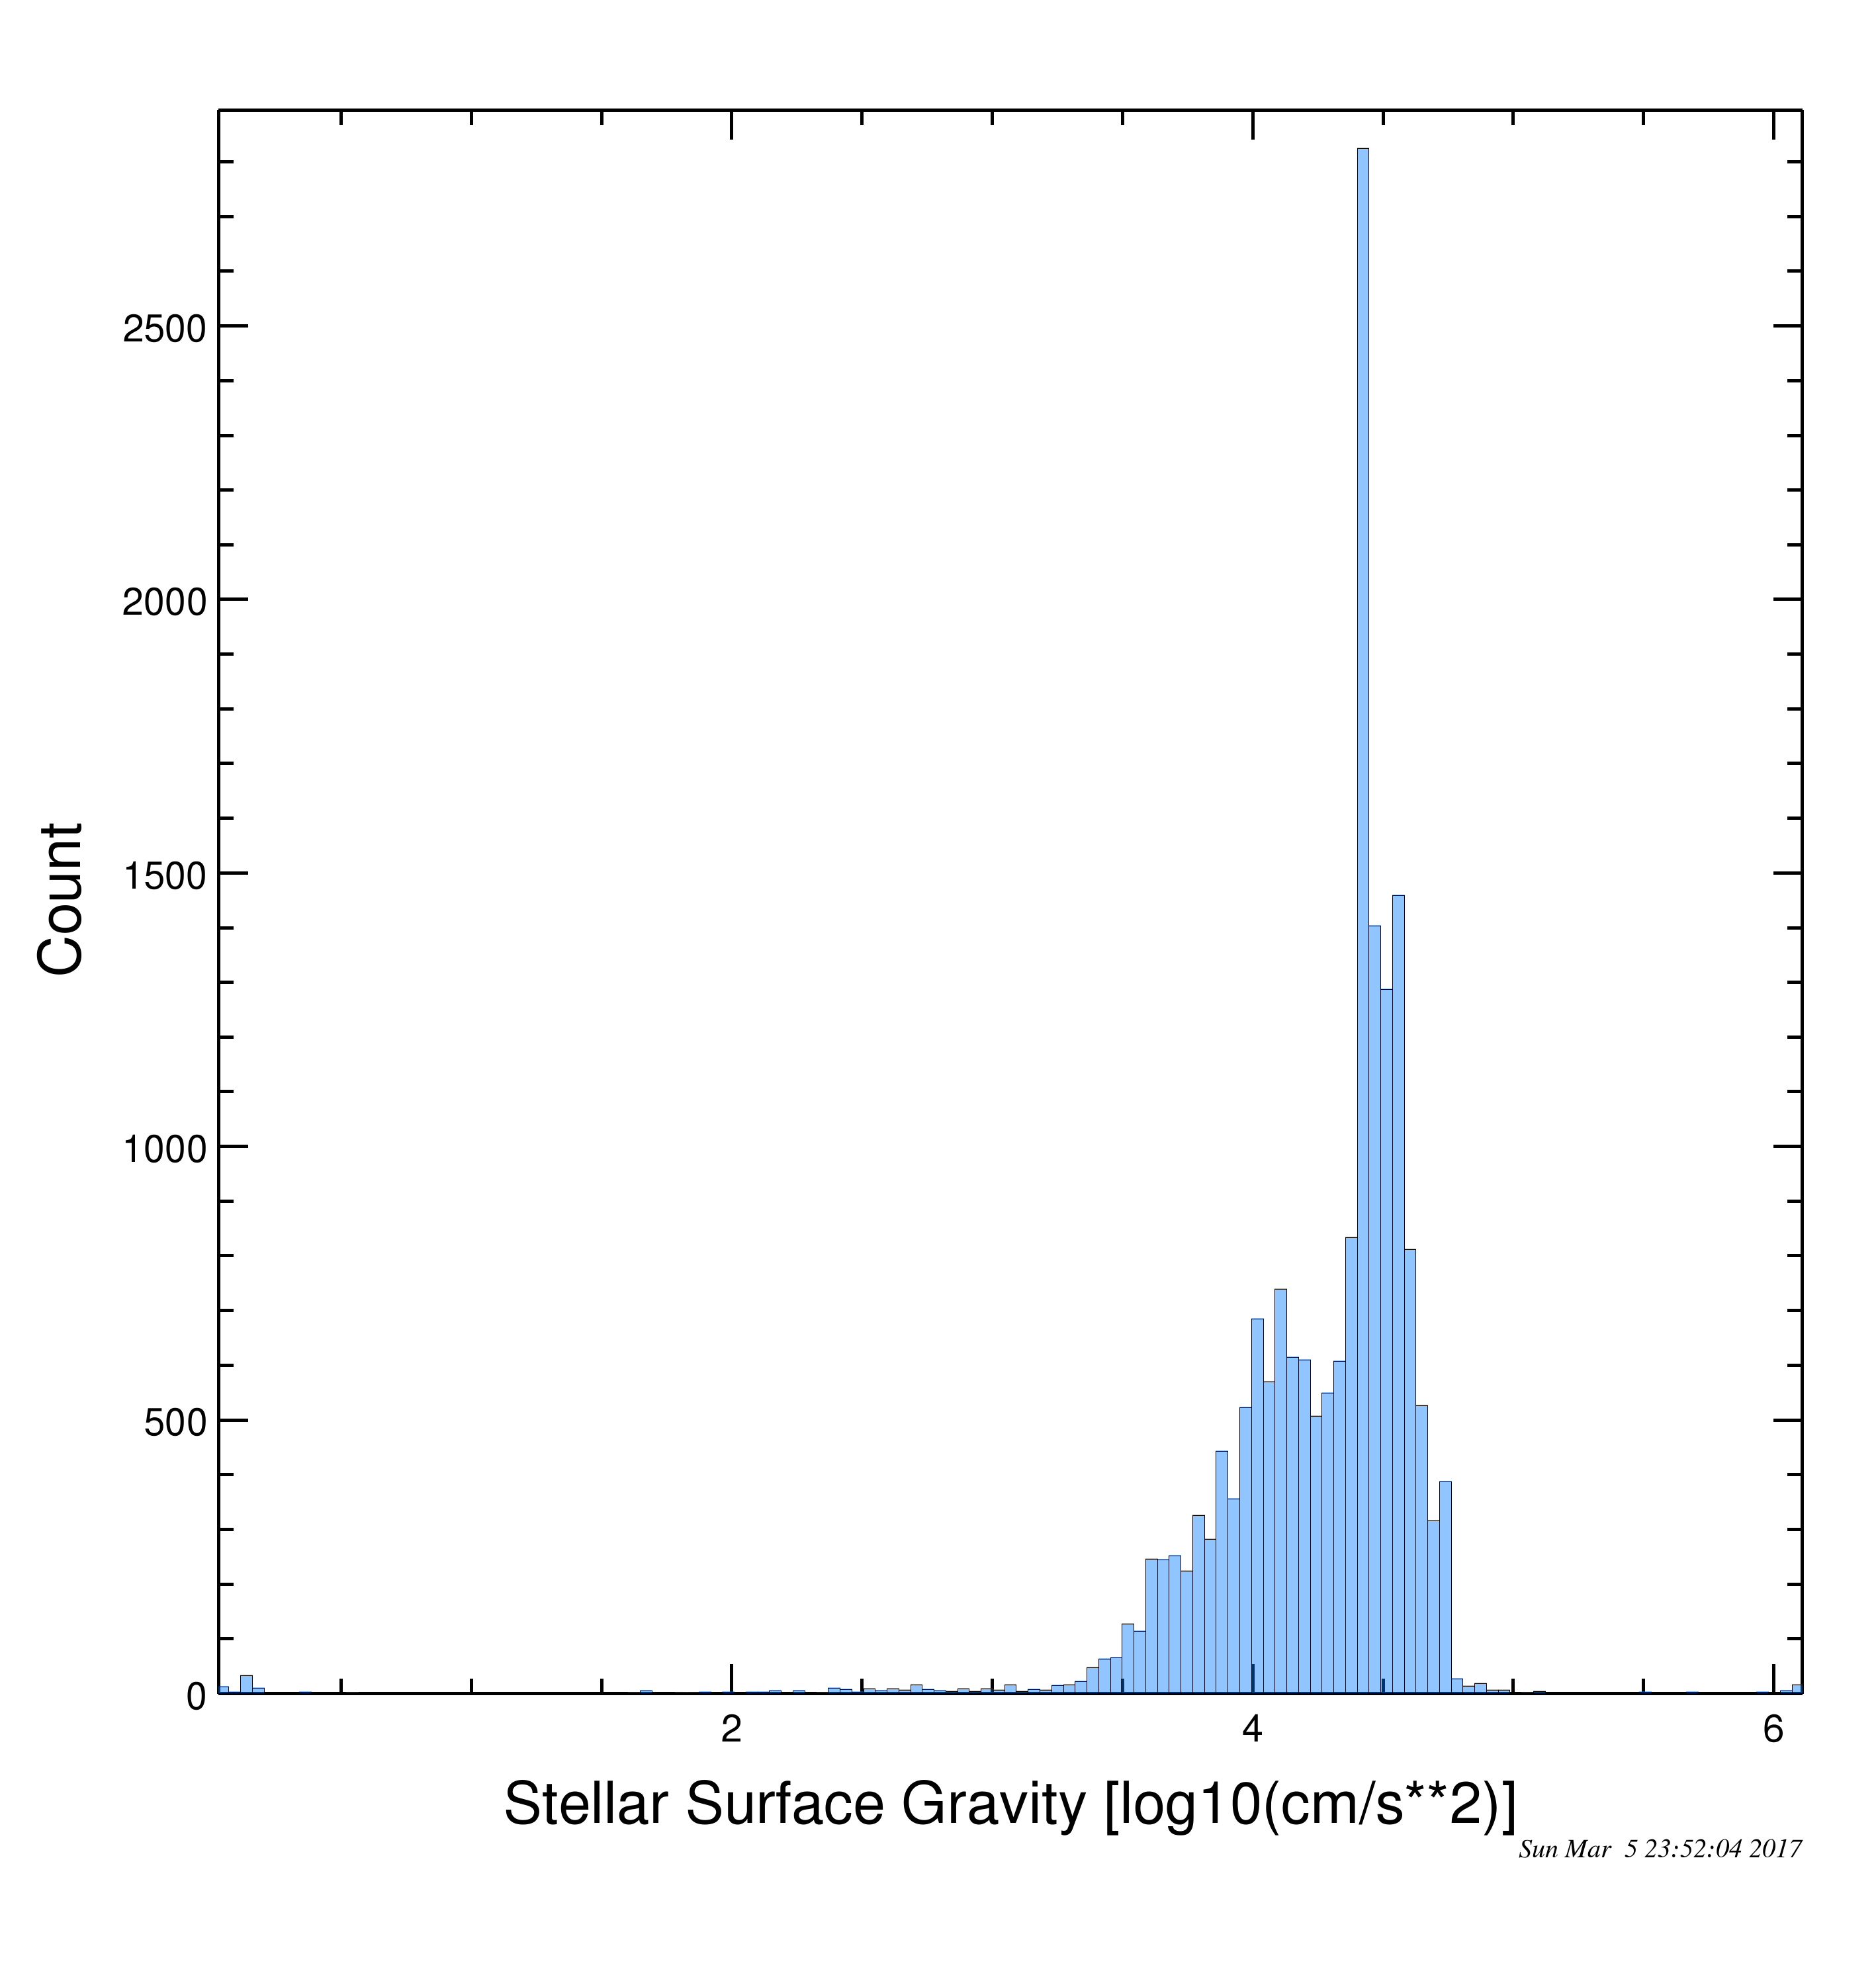
\includegraphics[width=0.5\textheight]{img/stellargravity.png}
        \caption{ Stellar Surface Gravity log10(cm/$s^{2}$)}  \label{plot:stellargravity}
\end{center}
\end{figure}

\subsection{Light Curve Based Vetting Statistics}
Kepler data pipeline performs detection tests using gap-filled flux time series. These time series usually build using multi-quarter data that observed by the spacecraft. In the process of combining these datasets, it removes edge effects around the data gaps and then combines the segments together. Gaps are filled by interpolating data segments.  TPS module of the pipeline estimates the Power Spectral Density of the flux tine series as a function of time. This generates coefficients for Single Event Statistics (SES) time series components. These can be interpreted as measurements fo the statistical significance of the presence of a transit of trial duration at each point in the time series. 

\subsubsection{Single Event Statistics (SES)}
The maximum calculated value of the SES. Maximum SES statistics for different TCEs from the same target differ because the most significant TCE is removed from the time series before repeating the test for further and weaker transit signals. 

\subsubsection{Multiple Event Statistic (MES)}
Multiple Event Statistic (MES) is the ratio of the detected signature's strength to the noise limit for a transit signature of the selected period and duration, or equivalently the SNR for the detection of the series of transits. This field contains the maximum calculated value of the MES.


\section{Missing Attributes}
In some circumstances, there are missing attributes in the dataset due to missing information in the stellar catalogs; the data validation fit fails to converge, or a processing timeout is reached. These missing attributes can be fill using reasonable methods such as mean, median, and in case of missing stellar attributes can be filled using sun's parameters. These various substitutions will be tested when training the network.


%\todo{Algorithms and Techniques}
%\todo{- Explain PCA indetail }
%\todo{- Explain CNN in detail}
%\todo{Benchmark - define the benchmark and thresholds - this is already done}

\section{Principal Component Analysis}
TCE attributes set contains well over 200 attributes. I use the Principal Component Analysis to reduce the dimention of this dataset. Principal Component Analysis (PCA) is a standard method use in modern data analysis. PCA provides a roadmap for how to reduce complex data set to a lower dimension to reveal the something hidden, and simplified structures that often underline it. PCA reduces the dimensionality of the data set while preserving most of the variation in data. This talk is accomplished by identifying directions, called Principal Components, along which the variation in the data is maximal. Using this method, a dataset that has a large number of variables can be express using fewer variables (components). 

\subsection{Naive Basis}
 The goal of PCA is to identify the most meaningful basis to re-express the data set while filtering out the noise and expose hidden structures. Lets assume we have a dataset with $m$ number of variables. We can represent these data set using a $m$ orthogonal basises. without loss of generality, we can visualize a data set with a 3 variables using $x, y, z$ axises. $x,y,z$ axises are being the vatiables (Figure \ref{plot:3d}). In other words, the basis of this dataset is {(1, 0, 0), (0, 1, 0), (0, 0, 1)}. We can raise the question why we need to pick this basis over any other basis? The reason is that the naive basis reflects the method we gathered data. We can express this naive basis using matrix as follows 


\begin{figure}[!h]
\begin{center}
        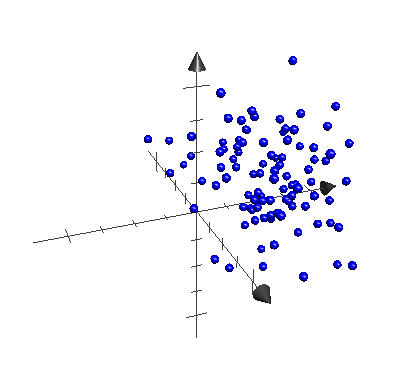
\includegraphics[width=0.4\textheight]{img/3D.png}
        \caption{Ax}  \label{plot:3d}
\end{center}
\end{figure}

\begin{equation}
%
    B =
	\begin{bmatrix}
    		b_{1}  \\
		b_{2}  \\
    		. \\
		b_{m}  \\
	\end{bmatrix}
	=
	\begin{bmatrix}
    		1 & 0 & 0 & \dots  & 0 \\
   		 0 & 1 & 0 & \dots  & 0 \\
    		\vdots & \vdots & \vdots & \ddots & \vdots \\
    		0 & 0 & 0 & \dots  &1
	\end{bmatrix}
	= I
%
\label{eq:I}
\end{equation}

Each row of this matrix is an orthonormal basis vector $b_{i}$ with $m$ components. All of our data has been recorded on this basis, and it can be expressed as a linear combination of ${b_{i}}$. Generalize form of the matrix can be written as a $m\times m$ identity matrix (Equation \ref{eq:I}).

\subsection{Change of Basis}

All the data has been recorded using naive basis; however, using linear algebra, we can find many other bases where these data can be re-express. For example, any rotation of naive basis will be perfectly valid basis to re-express the data. This is the question PCA precisely asking: Is there another basis, which is a linear combination of the original basis, which best re-express the data set?

Let us assume $X$ is our original data set and $Y$ is a new representation of the same data set.  We can perform a linear transformation ($P$) to produce $Y$ from $X$,

\begin{equation}
PX = Y
\label{eq:p}
\end{equation}

In matrix form, $P$ is a matrix that transforms $X$ into $Y$. Geometrically speaking $P$ rotate and stretch $X$ to produce $Y$. The rows of $P$ are a set of new basis vectors for expressing the columns of $X$.

\begin{equation}
%
    PX =
	\begin{bmatrix}
    		p_{1}  \\
		\vdots \\
		p_{m}  \\
	\end{bmatrix}
	\begin{bmatrix}
    		x_{1} & x_{2} & \dots  & x_{n} \\
	\end{bmatrix}
%
\label{eq:px}
\end{equation}

\begin{equation}
%
    Y =
	\begin{bmatrix}
    		p_{1}.x_{1} & \dots & p_{1}.x_{n} \\
		\vdots & \ddots & \vdots \\
		p_{m}.x_{1} & \dots & p_{m}.x_{n} \\
	\end{bmatrix}
%
\label{eq:y}
\end{equation}

Each column of $Y$ is a dot product of $x_i$ with the corresponding in $P$. Therefore, the rows of $P$ are a new set of basis vectors for representing of columns of $X$. 
It is important to mention that we are assuming the linearity and this reduce the problem to finding the appropriate change of basis. During this process, the row vector in the matrix P will become principal components. Now the question is what the criteria to pick the best possible basis P? The answer to this question is base on what features we would like Y to exhibit. 

Regardless the method of data analysis, the noise in the data must me low. If the noise in the data is significant, then the signal can not accurately extract.  The signal to noise ratio ($SNR$, Equation \ref{eq:snr}) or the proportion of variance sigma is high ($SNR >> 1$) for high precision data and low for noisy data.  best possible rotation for the naive basis is to find the basis that maximizes the $SNR$. This by assuming the dynamics of interest exists along directions with the largest variance. Therefore maximizing the $SNR$ allow us to find the best possible principal components. Finally, we can assume the Principal Components are orthogonal; this assumption provides an intuitive simplification that makes PCA solvable by using linear algebra decomposition techniques. 
\begin{equation}
SNR = \frac{\sigma^{2}_{signal}}{\sigma^{2}_{noise}}
\label{eq:snr}
\end{equation}

\subsection{Solving PCA using Eigenvalue Decomposistion}


One of the ways to find the PCA is using eigenvalue decomposition techniques. The first step is to find some orthonormal matrix $P$ (Eq \ref{eq:p}) by satisfying 
\begin{equation}
C_Y = \frac{1}{n} YY^{T}
\label{eq:cy}
\end{equation}


 $C_Y$is a diagonal matrix. The rows of $P$ are the principal components of $X$. Using simple substitutions using equation \ref{eq:p} and \ref{eq:cy}, we can derive $C_Y$ as, 

\begin{equation}
C_Y = P(\frac{1}{n}XX^{T})P^{T}
\label{eq:cy1}
\end{equation}

$\frac{1}{n}XX^{T} = C_X$ is the covariance matrix of X. Covariance matrix is a square matrix that has the variance of particular measurement types in diagonal terms, and off-diagonal terms are wth covariance between measurement types.  $C_X$capture the covariance between all possible pairs of measurements. Covariance values reflect the noise and redundancy in the measurements. In the diagonal terms, by assumptions, large values correspond to interesting structure, and in the off-diagonal terms, large values correspond to high redundancy. 

During the AVD, choice of $P$ diagonalizes $C_Y$. This was the goal of PCA. The results of the PCA can summarize as, 
\begin{itemize}
  \item The principal components of $X$ are the eigenvectors of $C_X$
  \item The ith components of $C_Y$ is the variance of $X$ along $p_i$
\end{itemize}


In practice computing PCA of a data set X is:

\begin{itemize}
  \item  Subtract off the measurement types
  \item  Computing the eigenvectors $C_X$
\end{itemize}


\section{Application of Artificial Neural Networks in Astrophysics}
In recent years, artificial neural networks (ANNs) have emerged as one of the potentially most successful modeling approaches in engineering and science. In this project, I am using backpropagation multilayered perceptron artificial neural network classifier to classify TCE catalog to identify planetary candidates. By using ANN, my objective is to apply machine learning technique to astrophysical datasets. 

ANNs are model after human brain and nervous system to simulate complex networks using interconnected modules. ANNs learn by examples; we call this a training data in which an actual measured set of input variables and the corresponding outputs are represented to determine the rules that govern the relationship between the variables. ANNs are well suited to modeling complex problems where the relationship among variables are not apparent and non-linear \cite{maier1995use}. The concept of artificial neurons was first introduced in 1943 \cite{mcculloch1943logical}, and since the back-propagation training algorithm for feed-forward was published in 1986 \cite{Rumelhart:1986:LIR:104279.104293}, ANNs has taken a significant advancement within last decade thus be considered as relatively new tool in the field of machine learning.

\subsection{Artificial Neural Networks}
ANN consists of a number of artificial neurons (also known as processing elements, nodes, or units). These neurons are usually arranged in layers. There are three different layers we can identify in ANN: an input layer, output layer and more layers between input and output collectively call hidden layers (Figure \ref{fig:ann}). 

\begin{figure}[!h]
\begin{center}
        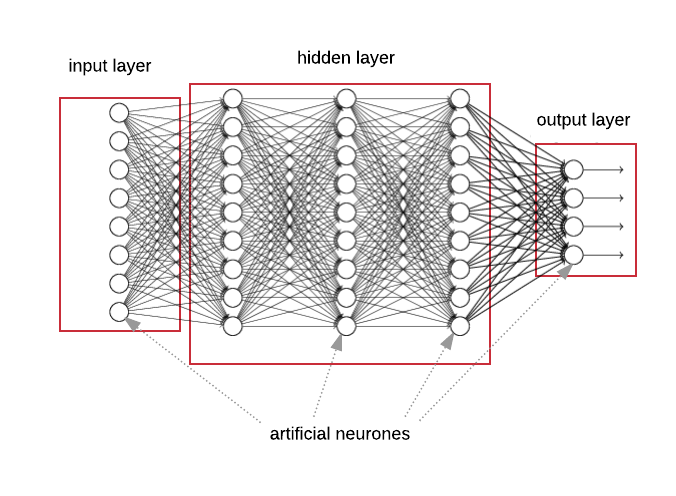
\includegraphics[width=0.7\textheight]{img/ann.png}
        \caption{Typical Structure of ANNs}  \label{fig:ann}
\end{center}
\end{figure}


\begin{figure}[!h]
\begin{center}
        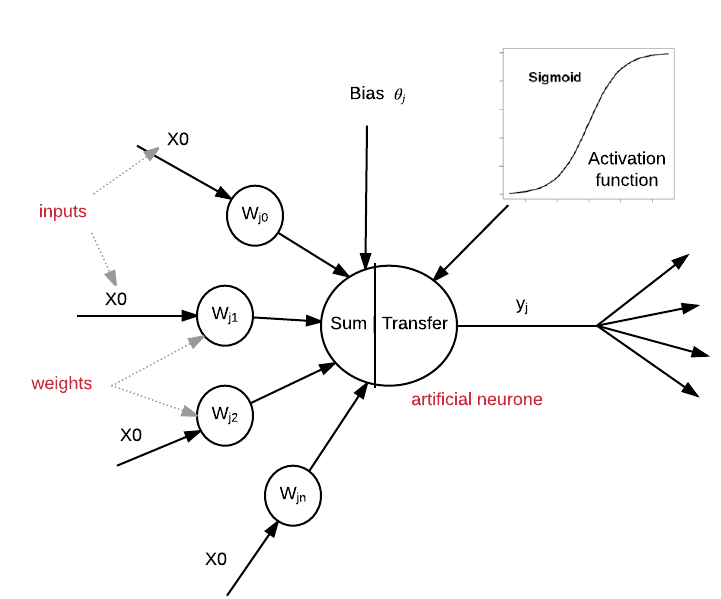
\includegraphics[width=0.6\textheight]{img/an.png}
        \caption{Artificial Neuron}  \label{fig:an}
\end{center}
\end{figure}

Each neuron is a layer partially or entirely connected to many other neurons via weighted connections. The scalar weights determine the strength of the connections between interconnected neurons. A zero weight means no connection between neurons and a negative weight refers to a prohibitive relationship. As shown in the Figure \ref{fig:an}, a neuron receives its weights inputs from other neurons which are summed, and a bias unit or threshold is added to subtracted. Bias us used to scale the input to a useful range to improve the convergence properties of the network (Equation \ref{eq:sum}).

\begin{equation}
I_j = \theta_j + \sum_{i=1}^{n} w_{ji}x_i
\label{eq:sum}
\end{equation}

Summed inputs $I_j$ pass through a transfer function to produce the output of the neuron. Figure \ref{fig:an} show this process for a neuron $j$ (Equation \ref{eq:transfer}).

\begin{equation}
y_j = f(I_J)
\label{eq:transfer}
\end{equation}

Using a predefined data set, that has known outputs for given inputs, and the network can be trained. The training steps are follows.

\begin{itemize}
\item Information propagation starts from the input layer where the data being fed to the network.
\item Inputs are weighted and received by each node in the next layer. 
\item Weighted inputs are summed and pass through a transfer function to produce neuron outputs, and pass to the neuron in the next layer. 
\item This process will be repeated while adjusting the weights to produce the predefined output of the training dataset. These weights are calculated by reducing the error.  
\end{itemize}


Learning in ANNs is usually divide into two separate groups: supervised and unsupervised \cite{mcculloch1943logical}.  Supervised learning neural network is given with a dataset with knows classifications (outputs), this dataset is known as the training data. During this project, I am using the supervised learning method to train the network. In this case, the network has been presented with TCE dataset with known planetary classifications. Network compare the known classification with the network output and compute the error. This error is used to adjust the weights among the neurons until the network produces the same results as the knows classifications in the training dataset. Two examples of Supervised learning ANNs are Multi-Layer Perceptrons (MLP) and neurofussy networks. In unsupervised learning, the network is only presented with the inputs without any desired outputs. The system itself adjusts the connection weights and cluster the input data records into classes of similar features.  ANNs also can be divided into two separate groups based on connection types among neurons: feedback networks and connections are in both forward and backward directions. During this project, I am using MLPs trained with a back-propagation algorithm. This has a high capacity of data mapping capabilities. 

\subsection{Multi-layer Perceptrons}
\label{sec:mlp}
In multi-layer perceptrons (MLPs) are fall under supervised feed-forward category in which the processing elements are arranged in a multilayered structure \cite{Introduction_to_the_theory_of_neural_computation} Figure \ref{fig:ann}.  As described in the equation \ref{eq:sum} and \ref{eq:transfer}, the input to a neuron is weighted and biased and run through an activation function before it passes on to the next layer. The output of a one neuron layer provides the input to the other next layer. The global error between the input and the output of the network is calculated using an error function. For example, the error function, for node j, is calculated using the equation \ref{eq:error}.

\begin{equation}
E = \frac{1}{2}\sum{(y_j - d_j)}^{2}
\label{eq:error}
\end{equation} 

where, $E$ is the global error function, $y_j$ is the predicted output by the network and $d_j$ is the desired output (from the training data set).

The objective is to minimize this error $E$ between the predicted and actual outputs. By reducing this error, the network can produce more accurate results. The minimization of this error function achieves with respect to all variables in the neural network such as connection weights, architecture, learning rate and threshold. Among these variables, connections weights are the most influential variable; thus back-propagation training algorithms are minimized the error function with respect to the connection weights only. Back-Propagation uses the gradient descent technique to adjust the weights in which the global error function, $E$ is minimized by modifying the weights using the equation \ref{eq:gd}.

\begin{equation}
\Delta{w_{ji}} = -\eta \frac{\partial E}{\partial w_{ji}}
\label{eq:gd}
\end{equation} 

where $\Delta{w_{ji}}$ is the weight increment from node $i$ to node $j$ and $\eta$ is the learning rate: the size of the step taken along the error surface is determined. 

The weights are then updated by adding the delta weight, xx to the corresponding previous weight as equation \ref{eq:weightupdate}

\begin{equation}
\Delta{w_{ji}}(n+1) = \Delta{w_{ji}}(n) + \Delta{w_{ji}}(n+1)
\label{eq:weightupdate}
\end{equation} 

where, $w_{ji}(n)$ is the value of the weight from node $i$ to node $j$ at step $n$ before the adjustment and $w_{ji}(n+1)$ is the value of the weight at step ($n+1$) after adjustment. 

\begin{equation}
\Delta{w_{ji}} = -\eta \frac{\partial E}{\partial w_{ji}} + \mu \Delta{w_{ji}}
\label{eq:momemtum}
\end{equation} 


First, the weights between the hidden and the output layers are adjusted, and then weights between the hidden layer and the input layers are adjusted. Learning rate is an another parameter we need to adjust in this process. Usually, the learning rate is adjusted by trial and error method. Smaller learning rate slows down the convergence even though the convergence can be achieved; however, it is subject to the local minima in the error surface that is closest to the random starting position. On the other hand, if the learning rate is large, the weight changes will be also large, causing the error to go up rather than down the thus convergence might never occur. However, larger learning rated might enable the model to jump out of local minima. Trial and error method to figure out the correct learning rate might lead us to oscillations, which can be overcome by adding another variable to the equation known as the momentum term ($\mu$). The process is to add a momentum term to the weight adjustment that is proportional to the amount of the previous weight change, Equation \ref{eq:momemtum}. Once the adjustments are carried out, it is saved and used to modify all the subsequent weight adjustments. This means that the weight change of the current step should carry some momentum of the weight change from the previous step. 

The process of adjusting weights is repeated until the network produce the desired results by minimizing the global error. Desired results are the output that given by the training data set. Once this process successfully calculates the proper weights, network continually can use these weights to make predictions, and at this point, we call this is a trained network that is ready to use in production. 

\begin{figure}[!h]
\begin{center}
        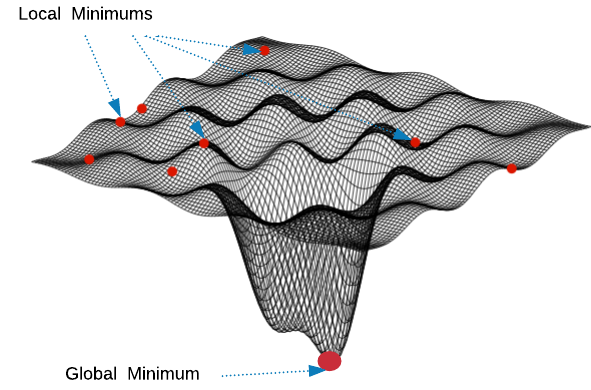
\includegraphics[width=0.4\textheight]{img/globalmin.png}
        \caption{Simulated error surface with local and global minimums. (Image credit: \url{https://projects.g-node.org/emoo/)}}  \label{fig:globalmin}
\end{center}
\end{figure}


Multi-layered perceptrons with back propagation algorithms are very efficient in many engineering problems; however, there are some limitations of this kind of neural networks. One of the limitation is that MLPs can get trapped in a local minimum in the process of finding the global minimum of the error surface. Exaggerated illustration of this issue is shown in figure \ref{fig:globalmin}. Gradient descent is working on reducing the error and trying to find the lowest error possible. As it shown in the figure  \ref{fig:globalmin}, there can be many local minimums presents in the error surface where the gradient descent may get trapped in local minimum even though there is a much apparent global minimum present.  In the literature, there are several ways proposed to escape from this local minima, including the learning rate, adding the momentum term, adding a small amount of random noise to the input patterns to shake the network from the line of steepest descent, adding more hidden nodes to relocating the network along the error surface by randomising the initial weights and retraining are some of them.Another limitation of MLPs is that feed-forward neural networks that are trained with the back-propagation are often criticized for being black boxes. The knowledge acquired by these networks during training is stored in their connection weights and bias values in a complex manner that is often difficult to interpret. 


To improve the performance of the ANN models,  we need to determine the model inputs carefully. Careful selection of the model inputs will significantly improve the performance of the network. Mostly we can choose the model input based on the prior knowledge of the problem we are aiming to solve. Another technique is to train many neural networks with different combinations of input variables and to select the network that has the best performance \cite{teh1997prediction}. There are many other techniques can be found in the literature to the best method to pick model inputs. Selecting a large number of input variables usually increase the network size resulting in a decrease in processing speed and reducing the efficiency of the network. 

Once the input parameters are selected, the dataset is divided into two separate sets: training and testing sets. Training set will be used to train and find out the connections weights and other network parameters by minimizing the error between model outputs and the corresponding measured values. Since ANN models have a large number of models parameters, this may cause to overfit the training data, especially if the training date are noisy. In other words, if the number of degrees of freedom of the model is huge compared to training date points, the model might no longer fit the general trend of the data. The testing data set used to make sure the model can generalize within the range of the data used for calibration. Usually, 2/3 of the data are recommended for a training dataset, and 1/3 will use as testing data.  If the available data are small, it is difficult to have enough data points in the training dataset hence the k-folding method can be used to separate dataset and train the network.  

Once the available data have been divided into training and testing, it is important to pre-process the data in a suitable form before they are applied to the ANN. Data pre-processing usually speed up the learning process. Pre-processing can be done in the form of data scaling (this allow the transfer function to perform well), normalization (in some cases the data need to be normally distributed to obtain optimal results) and transformation (transform the input data into some known form may be helpful to improve ANN performance). 


For free-forward neural networks, the most common method to find the optimum weight is the first order gradient descent. The advantage of this approach is that they have the ability to escape local minima in the error surface and thus produce optimal or near-optimal results. However, this also has a slow convergence rate. The stopping criteria are used to decide when to stop the training process. There are many criteria can be used to determine when to stop training: When the training error reaches a sufficiently small value. Or when not or slight changes in the training error occurred. However, the above example of stopping criteria may lead to the model ending permanently or over-training, and cross-validation approach can be used to overcome these problems. The cross-validation required to divide the data into three sets: training, testing and validating. 
 
\subsection{Model Validation}
The performance of the model validation ensures that the model has learned the complex and non-linear relations among variables using training data and is capable of generalized within limits. The standard approach is to achieve this is to test the performance of trained ANNs on the independent validation set, which has been using as part of the model building process. Prediction performance of ANN models are often evaluated using a couple of different methods: The coefficient of correlation (Equation \ref{eq:coefficient_of_correlation}) , root mean squared error (RMSE, Equation \ref{sq:rmse}) and mean absolute error (MAE, Equation \ref{sq:mae}).

\begin{equation}
r = \frac{C_{y_{j} d_{j}}}{\sigma{y_{j}\sigma_{d_{j}}}}
\label{eq:coefficient_of_correlation}
\end{equation}

where, $y_j$ - model (predicted) output, desired (observed) output, $C_{y_{j} d_{j}}$ covariance between the model output and desired output. Suggested values for $r$ are, 

\begin{itemize}
\item $|r| \ge 0.8$ - Strong correlation exists between two sets of variables. 
\item $0.2 < |r| < 0.8 $ - Correlation exists between eh two sets of variables 
\item $|r| \le 0.2$  - weak correlation exists between the two sets fo variables
\end{itemize}

RMSE is the most accepted measure of error and has the advantage that large errors receive much greater attention than small error.

\begin{equation}
RMSE = \sqrt{\frac{1}{n} \sum_{j=1}^{n}(y_j - d_j)^{2}}
\label{sq:rmse}
\end{equation}


\begin{equation}
MAE = \frac{1}{n} \sum_{j=1}^{n}|y_j - d_j|
\label{sq:mae}
\end{equation}

\subsection{Benchmark Model}

Benchmarking the neural network by performing many training trials by varying number of training data sets to reach the optimal network. Initial weight will be randomly chosen \cite{hamey1991benchmarking}. Comparing the performance of the NN with other classification algorithms also provide a degree of freedom to benchmark our model. In the literature there are many classification domains can be found that perform classification task on KOI dataset: K-nearest neighbors (K-NN) \cite{2011MNRAS.414.2602D}, Naive Bays \cite{feigelson2012}, Random Forests \cite{2015ApJ...806....6M}.

\begin{figure}[!h]
\begin{center}
        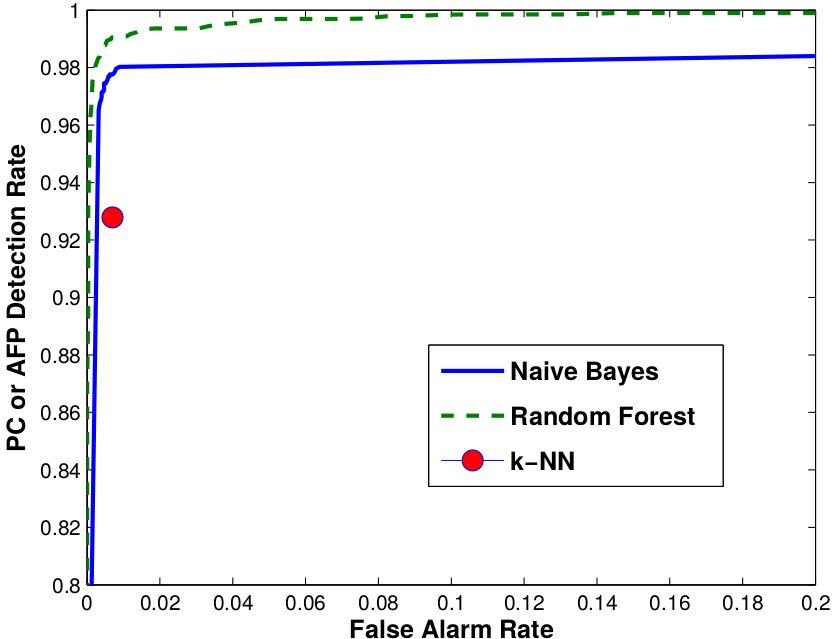
\includegraphics[width=0.35\textheight]{img/benchmark.png}
        \caption{Comparison of Random forest, Naive Bayes and K-NN. Image Credit: McCauliff et al. 2015 \cite{2015ApJ...806....6M}}  \label{fig:benchmark}
\end{center}
\end{figure}

Figure \ref{fig:benchmark} show PC or AFP Detection Rate vs False Alarm Rate of three different classification results performances. K-NN does not produce a ranking of predictions and so is represented as a single point in the plot. The resulting error rates for K-NN and Naive Bays are 3.15$\%$ and 2.73$\%$ respectively. I will be using these statistics that found in the literature as the benchmark for Neural Network using in this project.



% DONE
%\todo{Data Exploration}
%\todo{- Explain TCE Catalog in detail - show some samples, some of this already done}.
%\todo{- Explain the attributes in the dataset - may be use a table with detail description, try to visualize some of the attributes}
%\todo{- Missing data - from the paper, this is already done}
% TODO

%\todo{- remove the weak attributes}
%\todo{- Explain the classification labels in the dataset - this is already done}

\chapter{Methodology}

\todo{Data Preprocessing}
\todo{- talk about all the data preprocessings steps. PCA, and collect the the top 10 PCs and how that is define, show the table.}
\todo{Implementation}
\todo{- defien the trainng and testing data}
\todo{- Explain the cording process and any complications}
\todo{Refinement}
\todo{- Explain how the process improved. show the initial with someother activation function with bad outputs and bad loss funcitons. show some bad initial results.}
\chapter{Results}

\todo{Model evaluation and validation}
\todo{- Explain the final model paramters, explain}
\todo{- Explain the and show the loss funstion, show the confision matrix}
\todo{justification}
\todo{- Compare the final results to the bench mark - compare the confustion matrix to the once we have on the paper, also compare to the graph the score value, explain and show the problem is adiculately solved}
\chapter{Conclusion}

%\todo{Conclusion discussion - based on the conclusion section of the paper}
%\todo{Describe the entier process - highlight whats interesting and whats difficult, interesting - Astrophysics can replace the physical data processing piplelines with machine learning and allow real time dataprocessing with the large data comming from the telescopes}
%\todo{How can I Improve - this is where explain we can now do this using light curves instead using TCE catalog}

Machine learning techniques offer a way to automate some stages of the exoplanet discovery. In this project, I have demonstrated the backpropagated Multilayered Perceptron neural network is quite good at distinguishing between systematic noise, eclipsing binary and exoplanet candidates signatures from the TCE catalog. Within Kepler pipeline, there are plenty of statistical analysis methods have been using to scrutinize each light curve that is coming from Kepler spacecraft observation and also many other follow-up observations. Machine learning is something that has not been widely used in astrophysics. My primary goal is to introduce advanced machine learning techniques to analysis this astrophysical dataset that usually takes a much labor intensive process to automate. 

Workflow of this project as follows. NASA has a launch a spacecraft called Kepler in 2009 to observe a particular are of the sky for an extended period of time to understand the abundance of exoplanets, more specifically Earth-like planets. These observations are in the format of light curves. Light curves are build using the flux that coming from the star. These light curves have the flux fluctuations when planets are orbiting in front of the star. The fluctuations include other follow-up observations using many other ground and space-based telescopes. NASA has built a catalog called Threshold Crossing Event catalog (TCE) using this data. This TCE catalog further process using a pipeline called Kepler pipeline. During this pipeline, the data has been reduced to meaningful parameters where we can extract astrophysically interesting information. This catalog is available to for scientists to download for further studies. I have download this entire catalog from the NASA Exoplanet archives for this project. I have process this catalog and use the dimensionality reduction method (Principal component analysis) to reduce the dimensions of the dataset. The reduced data set then split into two sets: training and testing data. 

I have used the scikit learn machine learning package to build a backpropagation Multilayered Neural network (using python) and trained it using the training dataset. During this process, various parameters are tested to build a most appropriate neural network to analysis the TCE catalog. Once we build a well tuned neural network, I process the Kepler TCE catalog. This TCE catalog data is already scrutinized by a large number of scientists and also have done many follow-up observations using other telecopes to confirm the classifications. I was able to build a neural network to make this classification to 99$\%$ accuracy. Searching in the astrophysics literature, this is the first time anybody who used a neural network to make the classification for the Kepler dataset. 


As a next step, I am planning to advance this study further and introduce more machine learning into astrophysics world to accurately and quickly process data. Wtith the advancement of CCD technology and noise reduced electronics, and today telescopes produce much larger datasets within a short period with less noise. These data still being mostly analysis by manually by scientists and graduate students. With the help of machine learning, we will be able to build models where we can process these large datasets and make discoveries in much shorter timescales. It is vital for us to introduce these methods to expedite the data analysis process in astrophysics. Within this project, I am using the TCE catalog which is built by the Kepler pipeline using the light curves. I have proved that a simple neural network can process this dataset more accurately. As a next step, I am planning to advance further this study to build a machine learning algorithm pipeline to analysis the raw light curves that are coming from the spacecraft directly. Kepler mission has been completed; I will be able to use the existing lightcurve data and TCE catalog as my training dataset to build this platform where NASA and other fellow scientists will be able to use it to analysis the data from the future NASA missions that are scheduled to further advance the exoplanet hunts. It will be quite fulfilling see someday this work might help us to find extraterrestrial life. 

%\chapter{Problem Statement}

Kepler is a single instrument spacecraft that collect most contiguous and long-running photometric time series possible. Kepler has the capability to observe approximately 170,000 stars simultaneously while it is operating. The fundamental objective of the Kepler mission is to detect a large number of transiting exoplanets. The ultimate goal of the primary mission was a characterize the frequency of exoplanets on diameter, orbital period and host star.  The Manual classification of the findings of Kepler object has proven very time-consuming. The new space-based, transit photometry missions such as K2 \cite{2014PASP..126..398H}, TESS \cite{2014SPIE.9143E..20R}, and PLATO 2.0 \cite{2014ExA....38..249R} also produce a large number of the dataset that demands some level of automation to do the classification. 

Using machine learning classification techniques, we can speed up the process and provide a more continuous rating of planarity candidates. There are various of machine learning classification techniques has been applied to Kepler dataset including random forests, SVM, K-mean clustering \cite{2015ApJ...800...99T, 2015ApJ...806....6M}.  In this project, we are attempting to train a Multilayered Neural Network to identify the potential planetary candidates in the Kepler dataset. 

%\chapter{Datasets and Inputs}

\section{Kepler Pipeline}

The Kepler Pipeline \cite{2010ApJ...713L..87J} is a data reduction pipeline used for translating the Kepler raw pixel data into possible transiting planet detections. Kepler mission perform photometric observations of carefully selected stars (around 156,000) using its 115 deg$^2$ field of view (FOV) as reviewed in Borucki et el. (2010) \cite{Borucki977}
 and Koch et al. (2010)  \cite{2010ApJ...713L..79K}. The Kepler Mission Science Operations Center (SOC) at NASA Ames Research Center performs major functions on these datasets including calibrate CCD array, download data (light curves) from the spacecraft periodically, remove systematic noise \cite{2012PASP..124.1000S} and perform statistical tests to reject false positives and establish accurate statistical confidence in each detection.

\begin{figure}[!h]
\begin{center}
        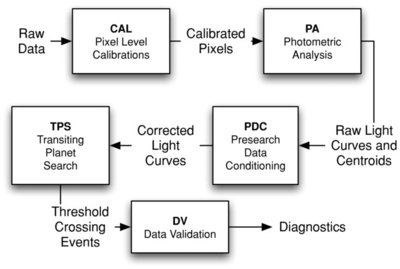
\includegraphics[width=0.5\textheight]{img/kpipeline.jpg}
        \caption{Data flow diagram for the SOC Science Pipeline. Image Credit: The American Astronomical Society}  \label{fig:kpipleline}
\end{center}
\end{figure}

Figure \ref{fig:kpipleline} show the major steps and modules of the pipeline. In particular the last two modules of the pipeline; those that identify as Threshold Crossing Events (TCEs) and their subsequent transit model fiting. TCE is a sequence of significant, periodic, planet transit-like features in the light curve of a target star. Transiting Planet Search module take takes as input the systematic error-correlated light curve for a star and searches a parameter space of possible transit signatures and outputs a TCE or say that does not exists TCE event on the target star. This produce smaller subset of target stars what is given to the Data Validation (DV) module. DV module takes initial TCE and gaps the transit signatures from the light curve and uses the Transiting Planet Search to find additional TCEs on the same target star. This process repeats until it finds all the TCEs on given star. More details on this process explained by Mandel and Agol (2002) \cite{2002ApJ...580L.171M} and Claret and Bloemen (2011) \cite{2011yCat..35290075C}.

TPS algorithm detects transit-like features in light curves by applying noise compensating, wavelet-based matched filtering. TPS characterized the power spectral density (PSD) of the observation noise as a function of time to implement a whitening filter in the wavelet domain. The trial transit pulse is whitened and correlated against the whitened flux time series. Features with correlations above the threshold of 7.1$\sigma$ are flagged as potential threshold crossing events and subjected to additional tests in TPS to guard against false alarms.

Algorithm searches a parameter space with varying transit durations $D$ and produce a Single Event Statistics (SES) time series that is the significance of the detection of the reference transmit pulse centered at that particular time for each $D$

\begin{equation}\label{eq:ses}
	SES(t) = N(t) /\sqrt{D(t)}
\end{equation}

$\sqrt{D(t)}$, is the expected signal to noise ratio of a signal that exactly matches the template pulse and $N(t)$ is the correlated time series.



Multiple Event statistics (MES) is constructed that characterizes a significant detection in a search over varying orbital period $p$ and epochs (phase) $t_0$ by folding $N(n)$ and $D(n)$. MES  $>$ 7.1$\sigma$ may produce a TCE if it also passes additional statistical tests. SES and MES are the basis of some of the attributes used in the training set.


\section{KOI and TCE Sttributes }

The Threshold Crossing Events (TCE) catalog contain a sequence of transit-like features in the flux time series of a given target star. These TCE data can download from NASA Exoplanet Archive databases \footnote{\url{http://exoplanetarchive.ipac.caltech.edu/cgi-bin/TblView/nph-tblView?app=ExoTbls&config=q1_q17_dr24_tce}}, and also the detail description of the table fields \footnote{\url{http://exoplanetarchive.ipac.caltech.edu/docs/API_tce_columns.html }} are listed as public data. Kepler Object of Interest (KOI) catalog contains object data including many attributes. The detail attributes are listed on NASA Exoplanet Archive website \footnote{\url{
http://exoplanetarchive.ipac.caltech.edu/docs/API_kepcandidate_columns.html}}, and dataset can be download from the arcive tables \footnote{\url{http://exoplanetarchive.ipac.caltech.edu/cgi-bin/TblView/nph-tblView?app=ExoTbls&config=cumulative}}. All these data cab be download as bulk using data tools available in the archive website.

\section{Some Important Attributes}
\label{label:important_attributes}
There are a large number of attributes available in the KOI and TCE datasets. Out of these attributes, following attributes has significant importance in classification process according to the literature. We will be including these attributes along side with other attributes that will be determined by using Independent Component Analysis.

\begin{itemize}
	\item $MES_{max}$/$MES_{min}$
	\item SNR (for all-transit model fit)
	\item MES scaled by SES auto-correlation statistics
	\item $\chi^{2}$ statistics for the all-transits model fit
	\item Ratio of the planet's semi-major axis to stellar radious
	\item The proportion of the light curve that was missing during this TCEs transit
\end{itemize}

\section{Missing Attributes}
In some circumstances, there are missing attributes in the dataset due to missing information in the stellar catalogs; the data validation fit fails to converge, or a processing timeout is reached. These missing attributes can be fill using reasonable methods such as mean, median, and in case of missing stellar attributes can be filled using sun's parameters. These various substitutions will be tested when training the network.

\section{Classification Labels}

Each Threshold Crossing Event (TCE) is subject to a vetting process performed by the Kepler TCE Review Team (TCERT). During the triage (Initial) vetting stage, all TCEs are partition into two different sets: Problematic Ligh Curves that has instrumental noise and Kepler Object of Interest. KOI is a TCE that contains convincing transit-like features that do not present obvious evidence that the TCE was generated from non-transiting phenomena such as instrumental noise. These KOIs moves to next level of the vetting process performed by individuals manually inspecting light curves using detection statistics. Any indication they see the signal came from an eclipsing binary star or more complex forms of instrumental noise removed from the list. TCEs that survive this removal process are classified as Planet Candidates (PC).


We can identify three different types of classification labels in the processed dataset: Planetary Candidates (PC), Astrophysical False Positives (AFP) and non-transiting phenomena (NTP). PCs are confirmed as planets, statistically validated as planets or determined to be a planet candidate by the TCERT. AFPs are those TCEs that have been shown to be eclipsing binary stars or have shown evidence that the transiting object being detected is not located around the target tart. NTP are those TCEs that failed the initial vetting process.

I am planning to use machine learning algorithm (Neural Network) to find a function that maps attributes produced by the Kepler Pipeline for each TCE to a classification label of PC, AFP or NTP. This classification funtion is purely based on the statistical distributions of the attributes for each TCE and the algorithm does not attempt to physically model the process of the planet transit beyond what is already present in the TCE attribute catalogs.

%\chapter{Solution Statement}


Machine learning techniques contribute a way to automate some step of exoplanet discovery. The TCE vetting process is a tedious and time-consuming (mostly a manual) process. Modern astronomical observational instruments generate a large amount of data within a short period of observational time. These observations may contain such a crucial events that need future follow-up observations using other telescopes (using other wavelengths); hence, processing these time series data and extracting meaningful information is a time sensitive process. Solution to this is to process Kepler data using machine learning algorithms to express the classification while reducing human errors. I am planning to use trained Neural Network to process the TCE data to make the classification. 
%\chapter{Benchmark Model}

I am planning to experiment with benchmarking the neural network by performing many training trials by varying number of training data sets to reach the optimal network. Initial weight will be randomly chosen \cite{hamey1991benchmarking}. Comparing the performance of the NN with other classification algorithms also provide a degree of freedom to benchmark our model. In the literature there are many classification domains can be found that perform classification task on KOI dataset: K-nearest neighbors (K-NN) \cite{2011MNRAS.414.2602D}, Naive Bays \cite{feigelson2012}, Random Forests \cite{2015ApJ...806....6M}.

\begin{figure}[!h]
\begin{center}
        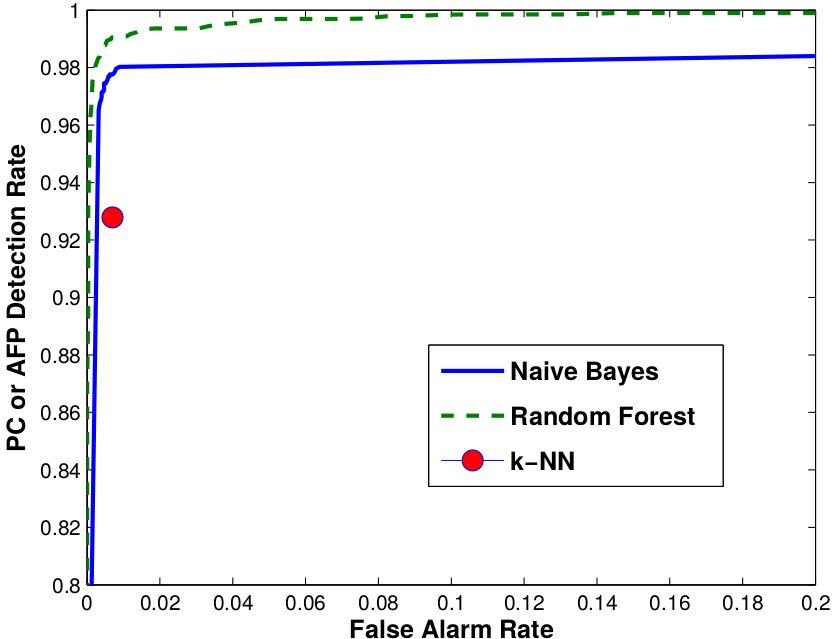
\includegraphics[width=0.35\textheight]{img/benchmark.png}
        \caption{Comparison of Random forest, Naive Bayes and K-NN. Image Credit: McCauliff et al. 2015 \cite{2015ApJ...806....6M}}  \label{fig:benchmark}
\end{center}
\end{figure}

Figure \ref{fig:benchmark} show PC or AFP Detection Rate vs False Alarm Rate of three different classification results performances. K-NN does not produce a ranking of predictions and so is represented as a single point in the plot. The resulting error rates for K-NN and Naive Bays are 3.15$\%$ and 2.73$\%$ respectively. I will be using these statistics that found in the literature as the benchmark for Neural Network using in this project.

%\chapter{Evaluation Metrics}

Using Neural network classifier to make classification on Kepler TCEs is a discrete prediction machine learning problem. That is to say; the NN decide what category the given TCE belong to. There are many metrics available for us to check how well our NN is performing and I am planning to use couple of these metrics in this project,

\emph{Mean Squire Error}, Attribute selection process will be using  Independent Component Analysis (as explain in the section \ref{label:important_attributes}) and MSE will use as the evaluation matrix for this stage.

\emph{Confusion Metrix}, will be as evaluation metrics for the NN. In confusion matrix, the columns indicate predicted classes, and rows indicates the actual classes. An entry in the diagonal shows the correct count classifications; off-diagonal indicates misclassifications of various kinds.

% \chapter{Project Design}

Theoretical workflow of the project 

\begin{itemize}
\item Download data from NASA Exoplanet archives 
\item Clean up attribute values 
	\begin{itemize}
		\item Understanding correlated attributes and remove them from final attribute set
		\item Produce additional Attributes
	\end{itemize}
\item Generate data into training, testing datasets. 
\item Develop a multilayered neural network using Python programming language 
\item Train the Neural Network 
\item Compare network results with the NASA Exoplanet Data
\end{itemize}

\bibliography{Reference/ref}
\end{document}



